\documentclass[a4paper]{article}

%% Language and font encodings
\usepackage[english]{babel}
\usepackage[utf8x]{inputenc}
\usepackage[T1]{fontenc}
%% Sets page size and margins
\usepackage[a4paper,top=2cm,bottom=2cm,left=2cm,right=2cm,marginparwidth=1.75cm]{geometry}
%% Useful packages
\usepackage{lineno}
\usepackage{amsmath}
\usepackage{graphicx}
\usepackage[colorinlistoftodos]{todonotes}
\usepackage[colorlinks=true, allcolors=blue]{hyperref}
\usepackage{natbib}
\usepackage{graphics}
\usepackage{mathtools,array}
\usepackage{float}
\usepackage{caption}
\usepackage{subcaption}
\usepackage{longtable}
\graphicspath{ {figures/} }
\usepackage{url}
\usepackage{caption}
\captionsetup{justification=raggedright, singlelinecheck=false}

\renewcommand{\baselinestretch}{1.5}
\setlength {\marginparwidth }{2cm}



\title{\vspace{3em}General Patterns in the Thermal \vspace{+1.7em} Responses of Microbial Lag and Exponential Growth Phases}
\author{Zongyi Hu}


\begin{document}


\begin{titlepage}

\newcommand{\HRule}{\rule{\linewidth}{0.5mm}} % Defines a new command for the horizontal lines, change thickness here

%----------------------------------------------------------------------------------------
%	LOGO SECTION
%----------------------------------------------------------------------------------------


\includegraphics[width=8cm]{title/logo.eps}\\[2cm] % Include a department/university logo - this will require the graphicx package
 
%----------------------------------------------------------------------------------------

\center % Center everything on the page

%----------------------------------------------------------------------------------------
%	HEADING SECTIONS
%----------------------------------------------------------------------------------------

%\textsc{\LARGE Project Dissertation}\\[1.5cm] % Name of your university/college
%\textsc{\Large Imperial College London}\\[0.5cm] % Major heading such as course name
%\textsc{\large Department of Life Science}\\[0.5cm] % Minor heading such as course title

%----------------------------------------------------------------------------------------
%	TITLE SECTION
%----------------------------------------------------------------------------------------

\makeatletter
%\HRule \\[0cm]
{\huge \bfseries \@title}\\[0.4cm] % Title of your document
%\HRule \\[0cm]
\vspace{+12em}
\begin{minipage}{0.4\textwidth}
\centerline{{\large \emph{Author:} Zongyi \textsc{Hu}}\\[1cm]}
\centerline{{\large \emph{    Aug 2021} }\\}
\vspace{+12em}
\end{minipage}
%----------------------------------------------------------------------------------------
%	AUTHOR SECTION
%----------------------------------------------------------------------------------------
%\begin{minipage}{0.4\textwidth}
%\begin{flushleft} \large
%\emph{Author:}\\
%Zongyi \textsc{Hu} \\ % Your name, if you are medically qualified please use "Last Name, M.D."
%[0.5cm] 
%\emph{CID:}\\
%02001365 \\
%[0.5cm] 
%\emph{Email:}\\
%zongyi.hu20@imperial.ac.uk
%\end{flushleft}
%\end{minipage}
%~
%\begin{minipage}{0.5\textwidth}
%\begin{flushright} \large
%\emph{Supervisor} \\
%Dr. Samraat \textsc{Pawar} \\% Supervisor's Name
%s.pawar@imperial.ac.uk \\
%[0.5cm] 
%\emph{Supervisor} \\
%Dr. James \textsc{Rosindell} \\ % Supervisor's Name
%j.rosindell@imperial.ac.uk\\
%[0.5cm] 
%\emph{Supervisor} \\
%Dr. David \textsc{Orme} \\ % Supervisor's Name
%d.orme@imperial.ac.uk\\
%\emph{Other Supervisors} \\
% \textsc{Add name here} % Supervisor's Name
% Supervisor Department(s) or NHS Trust+section
%\end{flushright}
%\end{minipage}\\[1cm]



% If you don't want a supervisor, uncomment the two lines below and remove the section above
%\Large \emph{Author:}\\
%John \textsc{Smith}\\[3cm] % Your name

%----------------------------------------------------------------------------------------
%	DATE SECTION
%----------------------------------------------------------------------------------------

%{\large \today}\\[1cm] % Date, change the \today to a set date if you want to be precise

\textsc{A thesis submitted for the partial fulfillment of the requirements for the degree of Master of Research at Imperial College London}\\[0.5cm]

\textsc{Submitted for the MSc in Computational Methods in Ecology and Evolution}\\[0.5cm]


\vfill % Fill the rest of the page with whitespace

\end{titlepage}


\centerline{IMPERIAL COLLEGE LONDON THESIS DECLARATION}
\bigbreak



I declare that this thesis represents my own work for the degree of Master at Imperial College London. It not substantially the same as any that I have submitted, or, is being concurrently submitted for other institution for a degree, diploma or other qualifications. \\

The data in this dissertation is provided to you by Samraat's laboratory, Department of Life Science, Imperial College London. \\
 
\linenumbers

% abstract
\begin{abstract}

% The goal of this project is to quantify the population growth pattern of microbes, the duration and pattern of the lag phase especially.
Microorganisms play a vital role in ecosystems globally. Microbial population dynamics is the fundamental process of microbiology, understanding it helps us learn more about the underlying metabolic strategies. While throughout the whole life cycle temperature takes a critical role in constraining the biological rates, recent studies do not take this constraint into consideration. With a deeper understanding of the thermodynamic constraints on metabolic traits, we could improve those models to a level with higher practical application value. In this study, I aim to find general patterns of temperature-related metabolic traits. By comparing the thermal responses within and across species, I find that the intensity of adaptation is stronger observed in the lag phase, which means the ability to surpass the thermodynamic constraint is higher in the lag phase. Under the same conditions, microorganisms spontaneously putting more effort into overcoming the thermodynamic constraint in the lag phase. This adaptive phenomenon leads to interesting questions about how the underlying mechanisms allocate limited resources in coping with changing environments to make the organisms more competitive.\\

%Why would this ability is stronger in lag phase than exponential phase? Would it also stronger than stationary or decline phase? Would the ability to overcome thermodynamic constrain be indication of higher competitiveness? what is the underlying mechanism makes microorganisms allocate the limiting resources to escape the thermodynamic constrains under constantly changing environmental conditions? All those questions are fascinating to explore and better understand the world, and me in this study, started with the base understanding of the thermal response of simple single population.
\end{abstract}



%%%%%%%%%%%%%%%%%%% 
\newpage
\tableofcontents

\newpage
\thispagestyle{empty}
\listoffigures
\listoftables
\clearpage
\pagenumbering{arabic}


%%%%%%%%%%%%%%%%%%% main %%%%%%%%%%%%%%%%%%% 
\newpage
\section{Introduction}

Microbes, as one of the earliest life forms, are ubiquitous on earth. They support all higher trophic organisms and maintain the health of the ecosystems \citep{whitman1998prokaryotes}. Their immense diversity, varied responses to environmental change and fast-changing generation features make it a valuable research model organism. Conversely, it is because of its complexity and diversity, studying every specific microbial system may be arduous and unrealistic. Therefore, exploring the common physiological mechanisms under microorganisms may give us more insights.\\
% and plays the vital role in producing foods, treating wastewater, keeping the etc.
% Influenced by the environment, while in turn make impact on their living environment. Understanding the interactions between them and the underlying response mechanism of the microbes can give back us more knowledge of the 

\begin{figure}[ht!]
\centering
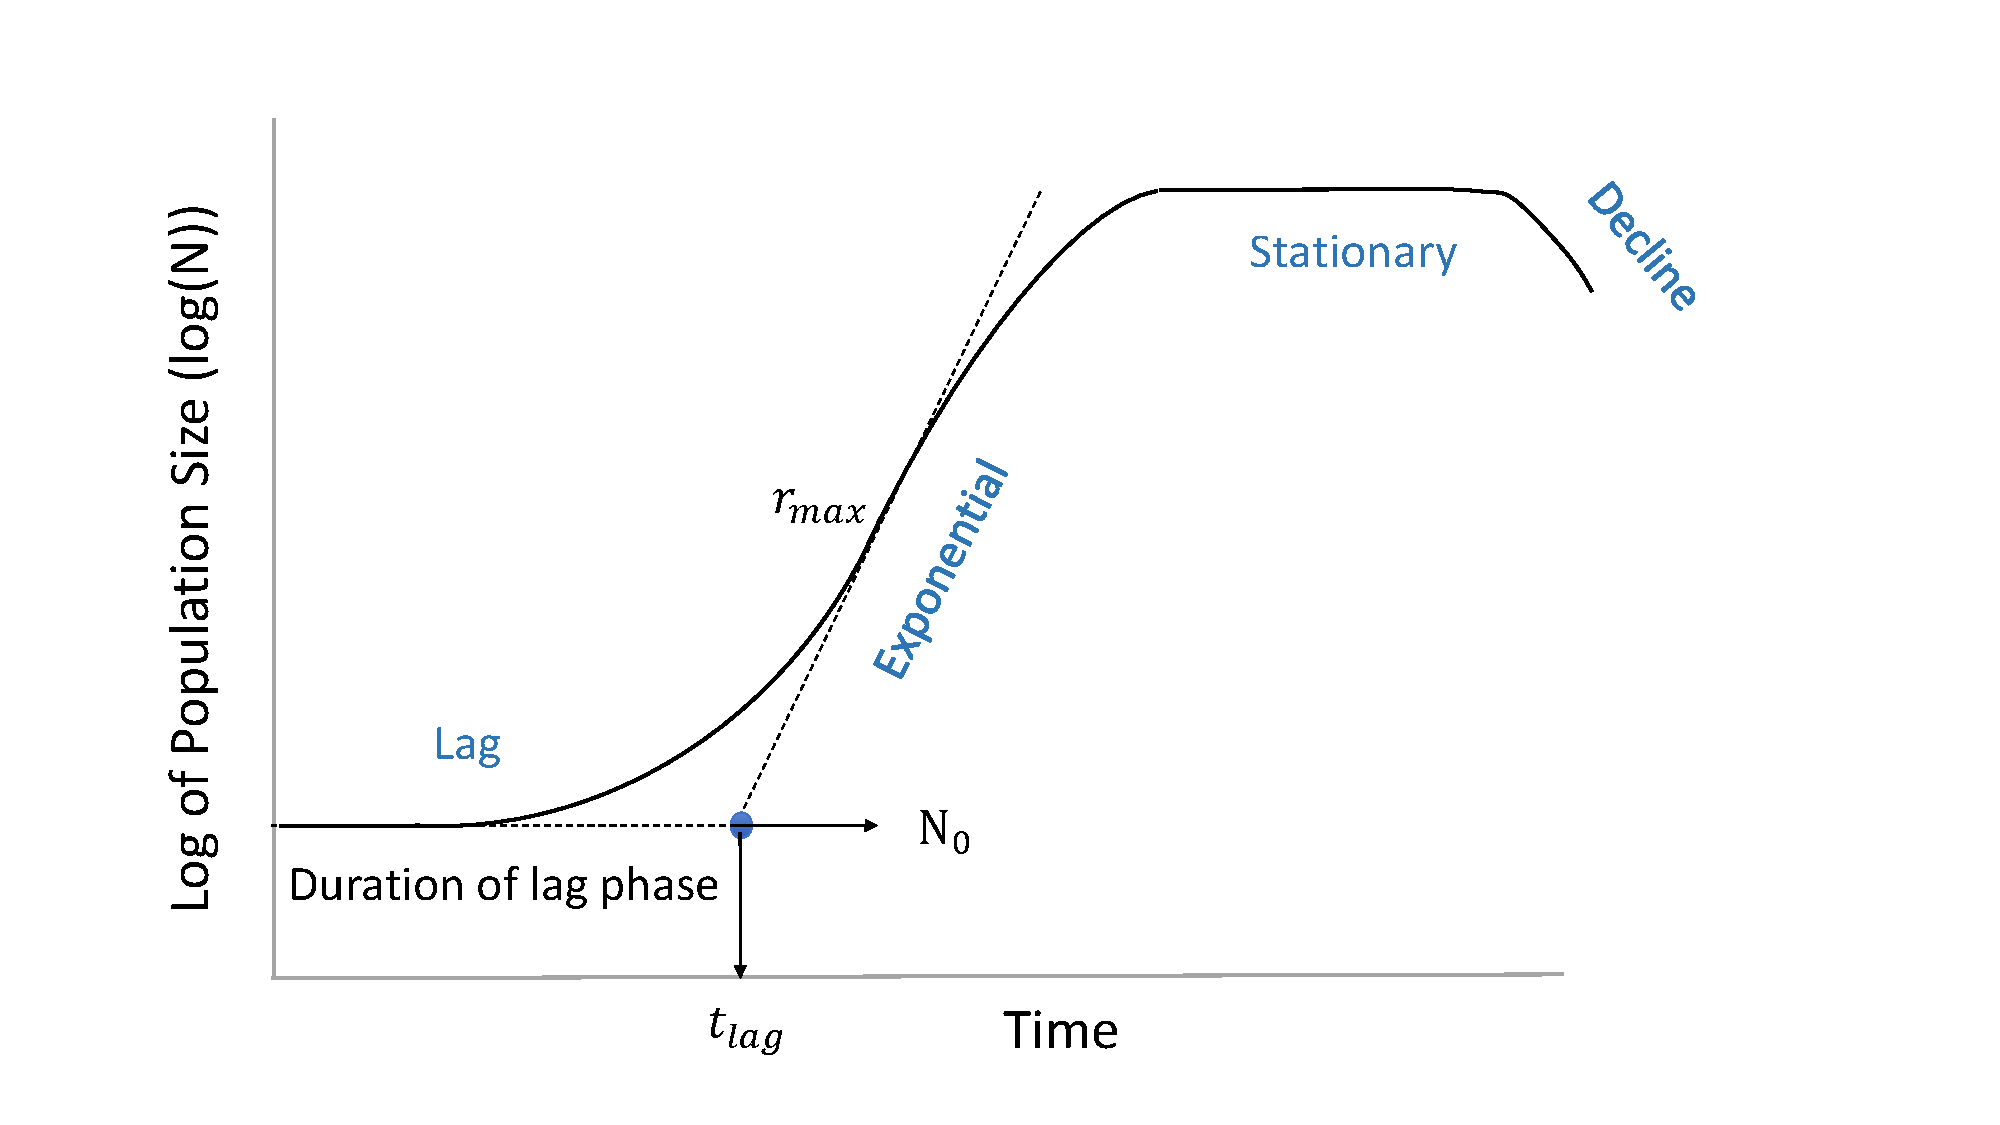
\includegraphics[width=0.95\linewidth]{Plot/typ_growth_pattern.pdf}
\caption{Typical Microbial Growth Pattern}\label{fig:typ_growth_pattern}
\flushleft{\normalsize Typical microbial growth pattern which can be divided into 4 phases: lag, exponential, stationary and decline phase. The sloped dashed line represents the maximum growth rate ($r_{max}$) which is the growth curve across the inflection point. This line intercept with the dashed horizontal line which shows the initial population size ($N_0$), gives back the blue dot has the x axis value defined as the duration of the lag phase ($t_{lag}$).}
\end{figure}
Microbial growth is a fundamental process in microbiology. Monitoring, interpreting and predicting the population growth of microbes inspire us to learn more about microbes. The growth curve of the microbial population can be divided into 4 phases (Fig. \ref{fig:typ_growth_pattern}): lag, exponential, stationary and decline. When encountering a new environment, microbes do not proliferate immediately, they adapt themselves to it. After this period, the population comes into its cell doubling phase. In this phase, the number of new individuals in the population appears to be proportional to the last generation. This proportion measured in the infinitesimal generation time interval, in the mathematical form $\frac{dN}{dt}$, is defined as the growth rate. The biggest growth rate at inflection point in this phase is defined as the maximum growth rate ($r_{max}$). The population cannot grow infinitely, and becomes relatively constant in the subsequent phase called the stationary phase. It may come about because of some growth-limiting factors, such as resources depletion. Due to the same or any other reasons like cell damage as stationary phase, when the fertility lies below the mortality, the population passes into the decline phase. \\
%In Fig. \ref{fig:typ_growth_pattern}, the dash line with the slope of the $r_{max}$ across the inflection point in the exponential growth phase of the growth curve intersect with the horizontal line with the y axis value of the initial population size, we get a point with the x axis value defined as $t_{lag}$, which represents the duration of the lag phase. 

In those growth phases, the intriguing phenomenon is that after inoculation, the microbial cells do not duplicate instantly. Although this was observed by Müller in 1895, after more than a century, there is still too little knowledge about them has been gained. Understanding the lag phase can deepen our understanding of microorganisms and have an application value \citep{bertrand2019lag}. For instance, the lag phase is commonly taken as the preparation period to respond to the changing environment and some suggest that microorganisms will repair some damage in the lag phase \citep{rolfe2012lag}. Understanding the strategies microbes take to cope with those damage or old cells may give back heuristic insight about ageing and longevity \citep{pin2009network}. The longer lag phase may help pathogens dodge the host immune responses, which confer increased antibiotic tolerance \citep{li2016importance}. Also, the seemingly maladaptive strategy of iron accumulation in the lag phase when the pathogen is exposed to antibiotics can reveal some underlying microbial regulation mechanisms and that instruct the use of antibiotics \citep{rolfe2012lag}.\\

Precisely modelling and predicting the growth pattern in the lag phase allows the modern refrigeratory food industry to preserve food from any organism contamination by prolonging the lag phase \citep{swinnen2004predictive,perez201318,ghidelli2018recent,adams2020microbiology}. Therefore we could boost the development of food safety and amplify the profitable fields of the food industry. In the food industry, the most commonly used and the main tool to suppress microbial growth in perishable foods is controlling temperature. In consideration of that, temperature with its critical influence on microbial metabolism \citep{brown2004toward}, provide a fundamental basis for understanding the latent mechanistic kinetic. Beyond that, the response of the soil microbes, because of the temperature perturbation, significantly influences the biogeochemical cycles \citep{davidson2006temperature}, which no creatures on earth could escape. \\
%among those factors that can influence the dynamics of the microbial population,  
%which is the primary measurement of the spoilage of the food, of any contaminating organisms present in the food, therefore. The  modeling and predicting the population growth gives food industry more informed knowledge about how to preserve food with any organism contamination from spoilage would   (double check).\\



\citealt{swinnen2004predictive} provided a framework explaining the mechanistic concept underlying the lag phase, which they define as a function of environmental change. The speed that microbes finish their work to adapt to the new environment can be expressed as $\frac{Workload}{\Delta time}$, in which $Workload$ is proportional to $\Delta Environment$, similar to \citealt{bertrand2019lag}. Recent work has shown that the duration of the lag phase is correlated to the rate of the environmental conditions change \citep{chu2016lag}. Facing the rapidly changing environment, the lag phase tends to be shorter and vice versa. From research by \citealt{chu2016lag}, we also get an insight into the microbial ability to adapt faster or grow faster. The authors believe that there is a trade-off between these two abilities. In which `grow faster' means microbe perform better in the subsequent exponential growth phase. However, as the research \citealt{chu2016lag} takes carbon source in the substrate as the environmental change, it is not clear that the same would be observed with the other environmental changes. Actually, the opposite result can be found in the study \citep{de2018determination} that there is not any trade-off between the ability to grow faster and adapt faster, rather they are positively correlated. Those microbes are studied under optimal growth conditions, except temperature and inoculation size as independent variables, monitored in the laboratory. However, in a recent study \citealt{hamill2020microbial} tried to explain the lag phase as the indicator of the stress, they claims there is no stable correlation between the length of the lag phase and the rate of growth or germination. \\


Based on the growth curve of microorganisms, is there a constant growth rate pattern? As growth rate is influenced by too many factors, such as temperature, body size, medium, inoculation size etc. It could be complicated and unrealistic to test each specific condition with an experiment. Rather than comparing the growth rate in specific conditions, there is a need to test it more generally using a mechanistic model to scale it into a generalized biological pattern. The Metabolic Theory of Ecology (MTE) \citep{brown2004toward} presents an approach. The MTE considers the dynamics of ecological systems as consequences of biological metabolism and deems the phenotypic variations within constraints on metabolic rate mainly influenced by body size, temperature and stoichiometry. In other words, most of the biological rates are governed by metabolism, so growth rate as a form of biological rate, could also be explained using MTE. \\

So far, there has been no research into the relationship between the lag phase and the exponential phase of microbes in terms of their short-term and long-term thermal responses taken into metabolism. It is therefore valuable to study the influence temperature has on the microbial growth dynamic of the lag and exponential phase focusing on the underlying metabolic relationship. In this study, I collected the microbial population growth data from Samraat Pawar's laboratory, the Department of Life Science, Imperial College. Those data are from 21 previous studies on microbial population growth that incorporated 94 species. By fitting the Boltzmann–Arrhenius model according to MTE, using data points within the Operational Temperature Range (OTR), we can get metabolic activation energy which represents the thermal responses of microbes in lag and exponential phase. \citealt{smith2019community} studied the adaptation by comparing the short-term and long-term thermal response of microbe using the maximum growth rate ($r_{max}$). I used the same method to compare the degree of adaptation between lag and exponential growth phases. I aim to infer some properties, for example, adaptability and potential metabolic mechanism, of microbes in the lag and exponential phases. \\
% not just comparing the growth rate under specific conditions which could be complex and unpredictable, can we by any means examining the underlying general mechanistic biological pattern and comparing the representative indicators to get more robust result?  1. at least chu2016lag say it could be a trade-off 2. chu2016lag say that just based on one study, it might not generally true 3. it could be complicated to do it more generally with an experiment 4. got data set to study, mention the lag size... 5. and need a  to explain it


% following up MTE, temperature is a critical confounding factor, that would affect maximum growth rate, duration of lag phase, in previous study did not taken into temperature...
% conversion the nutrients in the environment to biomass and maintain the base metabolism rate, the energy can represent the physiological status of the population[citation]\\
% Individuals within population undergo specific physiological responses during each phase for coping with the consistently changing environment. For understanding the thermal response of each phase, I consider quantifying the metabolism rates in lag and exponential phase. In this study, the rates are approximated by measuring duration of lag phase and take the reciprocal of this value as the transitional state growth rate ($t_{lag}$) and maximum growth rate ($r_{max}$) in exponential growth phase. For analysing the temperature effect on the metabolism rate of microbial growth follows the thermal-dynamic constrains can be quantified by the Arrhenius model \citep{peleg2012arrhenius} \\

%The specific metabolic properties of a microbe are the major factors in determining that microbe's ecological niche, and often allow for that microbe to be useful in industrial processes or responsible for biogeochemical cycles.\\

% Apart from reasons listed above can influence the duration of the lag phase, there are also some other explainations like...

% while recently there were already substantial evidence show that even genetically identical microbial has variation in the ability of adapting to the new environment, in the specific population \citep{vermeersch2019duration}. And 

% It can be influenced by the history of the microbes and the magnitude of the change between the preceding and the present conditions. and 'damaged' microbes always has longer lag phase\\

% after, there is still  when refers to a single cell, this period is defined as the from the inoculation till the first division. However, 

% As within this period, there is variation not only within the species of the biochemical, physiological and metabolic reactions but also exist among the population. The different transcriptomic, proteomic, and evolutionary features can also as the criteria of defining the lag phase.

% What causes the lag phase? What factors influence the duration of it? What can we infer from the phenomenon observed in the lag phase? Would longer lag phase mean better adaptation or opposite, and can we find the answer observing the subsequent exponential phase? Would there be any trade-off between the ability of adapt faster and grow faster? \\

%controlling temperature is the major means to preserve the food and delay the spoilage of the food, because it is the factor can influence both the duration of the lag phase and the maximum growth rate in microbes exponential growth rate \citep{}, within those two phase is the most effective duration can control the microbial growth. 

% After \citep{jacob1961genetic}, there have already loads of investigations towards explaining the mechanism underlying this phenomenon mostly focus on carbon source switches, but among those known or unknown mechanism, we know too little about what controls the duration of the lag phase \citep{yates2007lag}, which could have strong explanation power of adaptability of microbes. \\

%Why there are some individual differences regarding to the duration of the lag time? Would it represent the ability to adapt to the new environment? If one community adapt faster, can it grow faster or slower later on? \\

%It is reasonable to say, in order to out-compete other organism, it is beneficial to grow as fast as possible after inoculation, while there have already loads of phenomenon show that the duration of the lag phase can vary from minutes to years. Harsh environment can in some extend explain the very long duration of the lag phase, but how can we explain the relative slower individuals in adapting to a new environment? More confusing about it is why the variance exist among individuals with the identical gene within the same community? \\

%What is the most optimal strategy when a microbes move to a new environment? Would it be possible that some seems like sub-optimal strategy is actually the most optimal strategy for some reason say frequency dependent selection can act on it, or any drawback of it makes the benefit of employing sub-optimal strategy out-compete the cost of optimal one? \\

%%%%%%%%%%%%%%%%%%%%%%% Methods %%%%%%%%%%%%%%%%%%%%%%% 
\section{Methods}

I used the parameters $r_{max}$, $t_{lag}$ (Fig. \ref{fig:typ_growth_pattern}) as the real and reciprocal of the metabolic rate to estimate the thermal response ($E$) of microbes in exponential and lag phases. These metabolic parameters were obtained by fitting the modified Gompertz model. And the activation energy $E$ is by fitting the Boltzmann–Arrhenius model according to MTE. All the computation, analyses and plotting were done in R 4.1.1.\\
% fitted  and  to get parameters  and activation energy . And compared short-term (intra-specific, $\bar{E}_S$) and long-term (inter-specific, $E_L$) activation energy. 

\subsection{Data Collection}

The data were collected from 21 papers on microbial population growth under different abiotic conditions. The whole data set comprises around 94 species and across temperature range from -4$^{\circ}$C to 37$^{\circ}$C (for the detail refer to supplementary information \ref{Data_SI} on page \pageref{Data_SI}).\\

\subsection{Estimating Growth Rate Parameters}
\begin{equation} 
\label{eqn:GompEqn}
    log(N_t)= N_0 + (N_{max} - N_0) e^{-e^{r_{max} exp^{(1)}  {\frac{t_{lag}-t}{(N_{max}-N_0)log(10)}\\} +1}}
\end{equation}
The modified Gompertz Model \citep{zwietering1990modeling} is wildly validated as an appropriate model, which is frequently used to describe the growth of population and each parameter in the equation has biological meaning. Therefore, I use it to estimate the two metabolic rate parameters: $r_{max}$ and $t_{lag}$, which are taken as fitness measurements in this study too. \\

Before fitting the Gompertz model, I deleted data with incorrect species names and with negative population sizes, which do not have biological meanings. Then, as the model has used the logarithm of population size, I also deleted the population size that has the value of 0 and takes the logarithm of it ($log(N)$). And for fitting the model, it also requires a sufficient degree of freedom in each fitting. There are 4 parameters in the Gompertz model (equation \ref{eqn:GompEqn}), so the data set that has less than 5 points were also deleted. Moreover, each fitting means fitting the model on each data set under the same experimental conditions. So the ID value contains information of species, medium, temperature and citation is given to each data point. The data points with the same ID value are taken as a data set. After the above steps, 809 valid data sets could be used in model fitting.\\

The model was fitted using Non-linear Least-squares, \texttt{nlsLM()} function in R based on the Levenberg-Marquardt algorithm. The estimated parameters in fitting the Gompertz model (equation \ref{eqn:GompEqn}) were sampled 1000 times and retained the parameters in the fitting with the minimum AIC value. The AIC value is a criterion for evaluating the goodness of fit. \\
% this project to estimate the maximum growth rate $r_{max}$ and lag phase growth rate $t_{lag}$, taken as the direct measure of fitness of microbes in exponential and lag phase respectively in this study, by fitting the  so that each parameters in equation has biological meanings. Among those parameters, I use $r_{max}$ and $1/t_{lag}$ to represent the growth rate of the lag and exponential phase. \\

% In this study, the modified Gompertz \citep{zwietering1990modeling} model was used to fit and generate estimated lag and exponential phase fitness, the growth rate of the two phases($t_{lag}$ and $r_{max}$). And for researching the thermal response of those two phase, I follow the method used in this study \citep{smith2019community} using the Arrhenius model by considering the physical chemistry kinetic factor of inferring the thermodynamic status of the population. After fitting the model, I can get the thermal sensitivity value ($E_a$, E hereafter) of both stages and by comparing the activation energy patterns shown within and across species and examining the short- and long-term of the thermal response of the patter observed across species, the relationship between the lag and exponential phase can be obtained and further inference about the competitive ability of different strains.\\

\subsection{Determining the Operational Temperature Range}
The organisms have their own Operational Temperature Range, studying their metabolic rate out of this range does not provide too much practical significance. And also the Arrhenius model would not be applicable out of the bound, for it requires the reaction rates to increase monotonically with temperature \citep{peleg2012arrhenius}. The normal temperature range for most organisms falls into 0 to 40$^\circ$C \citep{thompson1942growth} and I scatter plotted the growth rates changing V.S. temperature. By roughly examining the general trend of it, I take 30$^\circ$C as the upper limit of the operational temperature range.\\
% plotting population growth rate in lag$(t_{lag})$ and exponential($(r_{max})$) phase corresponding to the value of $\frac{-1}{K T}$ respectively (see detail in SI). Visual the curvature change trend \ref{fig:mean_rate_temp_group}, \\



\subsection{Calculating the Activation Energy}

The MTE equation (equation \ref{eqn:MTE}) builds on allometric equations (equation \ref{eqn:allo}) \citep{kleiber1932body} and the Boltzmann–Arrhenius model (equation \ref{eqn:ArrheEqn}) that explains the mass- and temperature-correlated rate respectively. However, studies have already proven that only mass-specific metabolic rates change in response to temperature \citep{schramski2015metabolic}. So the mass-specific rate of metabolism $B$ scales as the equation \ref{eqn:MTE_mass} by dividing $M^{\frac{3}{4}}$ on both sides of the equation \ref{eqn:MTE}. \\
\begin{equation}
    \label{eqn:allo}
    Y = Y_0 M^{\frac{3}{4}}
\end{equation}
\begin{equation}
    \label{eqn:ArrheEqn}
    B = B_0 e^{-\frac{E_a}{k T}}
\end{equation}
\begin{equation}
    \label{eqn:MTE}
    I = I_0 M^{\frac{3}{4}} e^{-\frac{E}{k T}}
\end{equation}
\begin{equation}
    \label{eqn:MTE_mass}
    B = B_0 M^{-\frac{1}{4}} e^{-\frac{E}{k T}}
\end{equation}
% Van’t Hoff-Arrhenius model

This dissertation takes temperature as the critical confounding factor, so incorporate the $ M^{-\frac{1}{4}} $ into constant $B_0$ in equation \ref{eqn:MTE_mass} comes to the same pattern as Boltzmann–Arrhenius equation \ref{eqn:ArrheEqn}, the actual model being fitted. So that $B_0$ is the normalization constant independent of body size, temperature and other abiotic factors. $Y_0$ in equation \ref{eqn:allo} and $I_0$ in equation \ref{eqn:MTE} are also constants. $B$ in equation \ref{eqn:ArrheEqn} is explained as the frequency that the collisions result in a reaction. Under this specific dissertation, it is taken as the mass-specific biological growth rate under consideration of MTE. $Y$ in equation \ref{eqn:allo} and $I$ in equation \ref{eqn:MTE} represent whole-organism metabolic rate.  $E_a$ is the apparent activation energy, correspondingly $E$ is the metabolic activation energy. $K$ is the Boltzmann constant, $T$ is the absolute temperature in Kelvin. \\

In the same circumstance as the Gompertz model, the log transformation process and sufficient degree of freedom requirements need to be handle. Those two metabolic trait parameters, $r_{max}$ and $1/t_{lag}$, were log-transformed. Before that, non-positive estimated parameters were deleted. Each within species fitting used the data sets with the same species, more than one temperature and more than 2 data points data sets. The across species fitting used the highest metabolic rate parameters in the fitting within species. Both fitting used \texttt{lm()} function in R 4.1.1. \\
\begin{equation}
    \label{eqn:logArrheEqn}
    ln(B) = ln(B_0) - \frac{E}{k T}
\end{equation}



\subsection{Comparison of Thermal Response Patterns}
\begin{figure}[!htb]
\centering
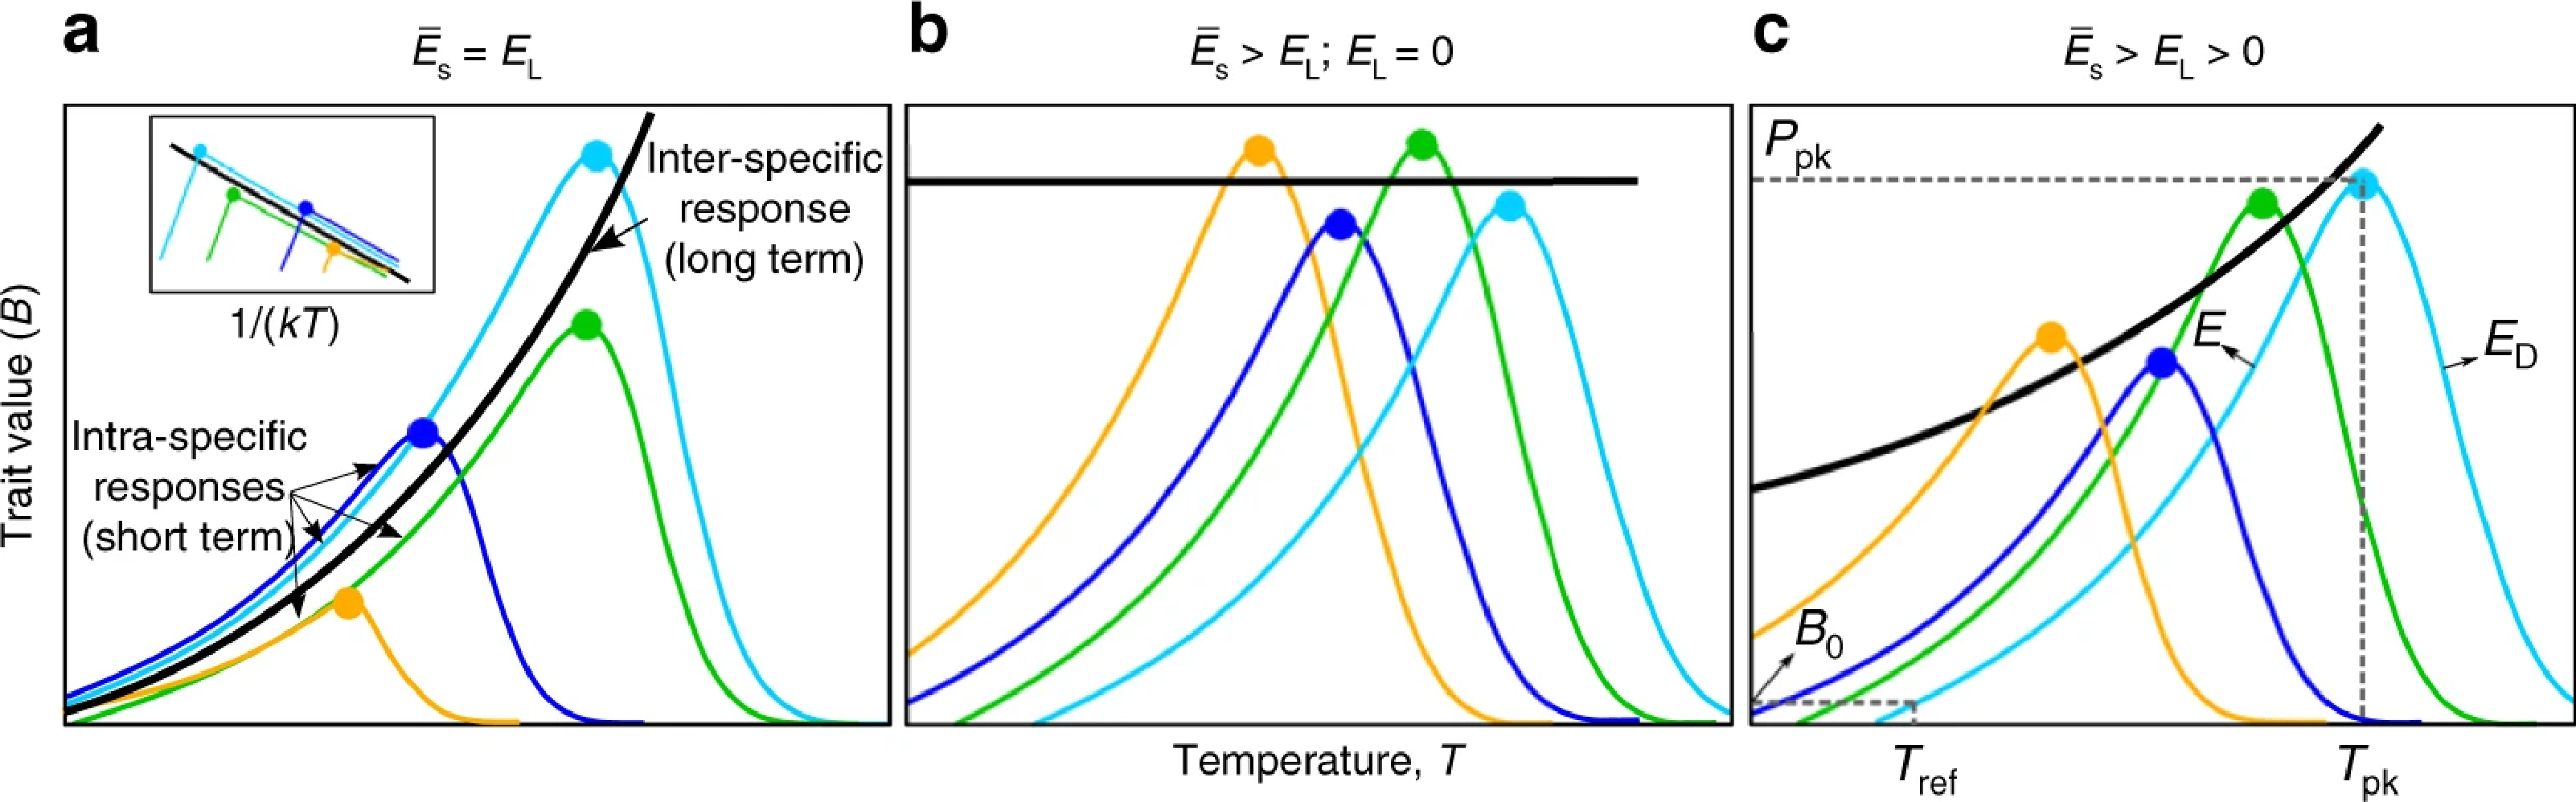
\includegraphics[width=0.95\linewidth]{Plot/E_short_long_cite.pdf}
\caption{Thermal Response Patterns}\label{fig:E_short_long_cite}
\flushleft{\normalsize copy from \citep{smith2019community}. The coloured lines are intra-specific Thermal Performance Curve (TPC) used to calculate intra-specific activation energy, which represents the short-term thermal response. The black line, using only the trait value under the optimum condition ($P_{opt}$) to generate inter-specific activation energy, corresponds to long-term thermal response. Inset panel in a shows how the plot would be like in the Boltzmann-Arrhenius model. $\bar{E}_S$ is the mean intra-specific activation values (the absolute values of the slope of the colored lines in panel plot), correspondingly $E_L$ is the black line. Larger activation energy value represents larger thermal constrains (larger thermal sensitivity), short-term. So by comparing the difference of the short-term and long-term activation energy, we can infer the degree of the adaptation. In this plot, the three circumstances are: \textbf{a} there is no adaptation, the short-term activation energy ($\bar{E}_S$) is statistically indistinguishable from the long-term (${E}_L$). The metabolism rate is completely constrained by the thermodynamic \textbf{b} Natual selection defeats thermoconstrains completely. \textbf{c} Intermedium senarial that the microbes is partialy adapted.}
\end{figure}
The estimated parameters $log(1/t_{lag})$ and $log(r_{max})$ are scatter plotted to get an overview of the general relation between them. The regression line was gotten by using the 'loess' method in the ggplot2 package with 95\% prediction bounds. Then, a more precise quantitative comparison is exerted to get the activation energy by fitting the Boltzmann-Arrhenius model.\\

As shown in Fig. \ref{fig:E_short_long_cite}, the short-term ($\bar{E}_S$) and long-term (${E}_L$) activation energy in both lag and exponential phases had been computed and compared to infer the thermal sensitivity and the degree of adaptation in each growth phases. Each short-term Arrhenius fitting used the data set with the same species and got the short-term activation energy $E_S$. Intra-specific (short-term) thermal response ($\bar{E}_{S}$) of microbes were calculated by taking the average of intra-species activation energy $E_S$. The long-term fitting used the data points across species, each at the optimal temperature in the short-term fitting. The optimal temperature at which these data points are located has the largest average growth rate in each short-term fitting. \\

% Es EL can also taken as average rate? 
% Conclusion: the metabolic rate in lag phase is more constrained by thermodynamic. what does the E from MLE mean, underlying?

% If the temperature before changing is already the optimal temperature leading to optimal growth rate, the natural selection would select the individual with lower activation energy, so that, it would not influenced by the temperature perturbation too much? but the thermal constraints within species is hard to evolve. So adopt the explanation above!\\


%%%%%%%%%%%%%%%%%%%%%% Results %%%%%%%%%%%%%%%%%%%%%% 
\section{Results}

% 1
\subsection{Correlation Between Growth Rate Parameters}

By plotting metabolic rate parameters of exponential phase ($log(r_{max})$) and lag phase ($log(1/t_{lag})$) (Fig. \ref{fig:log_rt_col_temp}), it shows a positive correlation between those two parameters. \\

\begin{figure}[ht!]
\centering
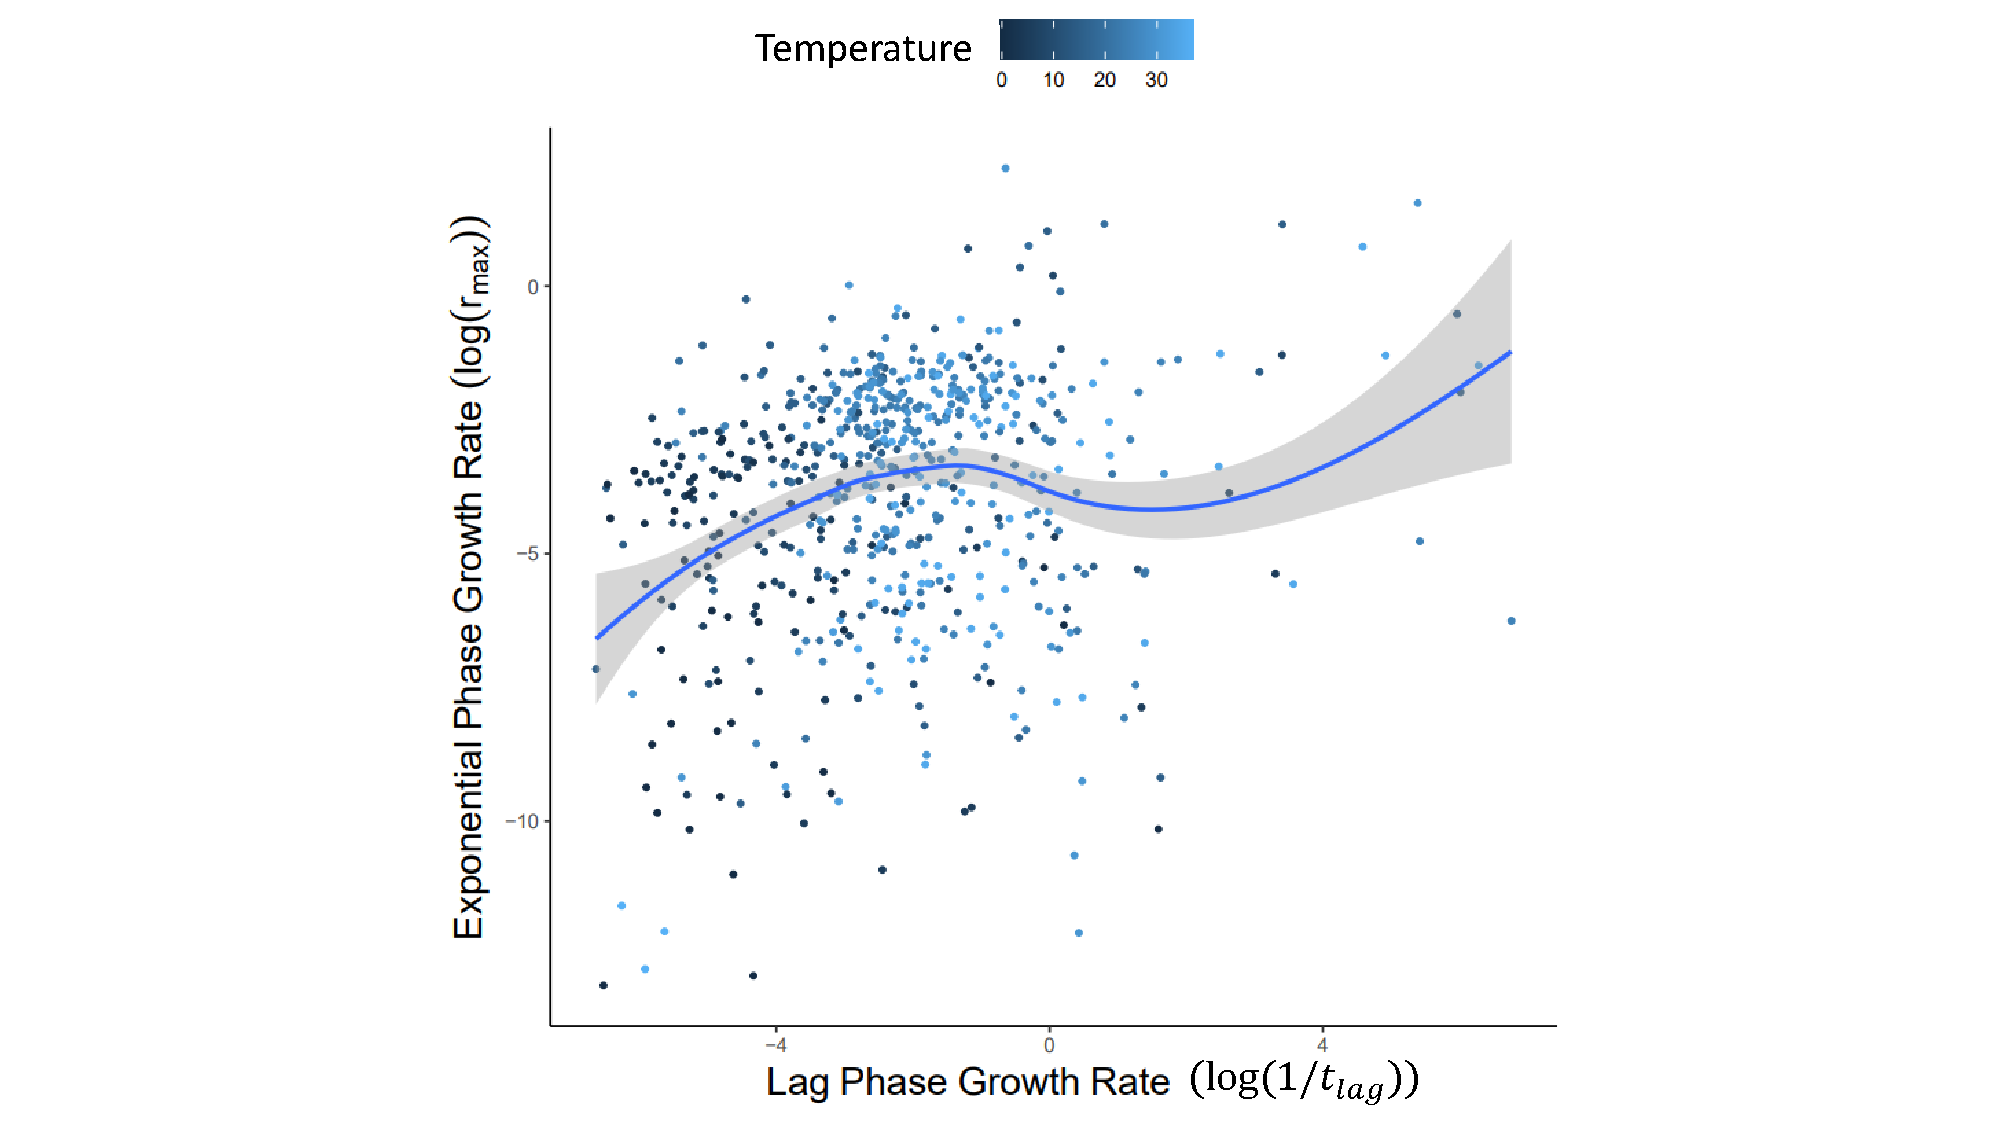
\includegraphics[width=0.75\linewidth]{Plot/log_rt_col_temp.pdf}
\caption{Rough correlation between metabolic traits}\label{fig:log_rt_col_temp}
\flushleft{\normalsize The correlation between metabolic rate parameters of exponential and lag phases under different temperature. The regression line is fitted using 'loess' method in ggplot2 package with 95\% prediction bounds.}
\end{figure}

% 2
\subsection{Operational Temperature Range}

%Across species log of maximum growth rate ($log(r_{max})$, left) and log of lag phase growth rate($log(\frac{1}{t_{lag}})$, right) corresponding to the value of $\frac{-1}{KT}$}
Visually, the data with the temperature above 30$^{\circ}$C would largely not follow the Arrhenius model that the reaction rate increase monotonically with temperature (Fig. \ref{fig:rate_temp}, \ref{fig:mean_rate_temp_group}) \citep{peleg2012arrhenius}.  So I take 30$^{\circ}$C as Operational Temperature Range upper bound.\\

\begin{figure}[ht!]
\centering
    \begin{subfigure}{.47\textwidth}
      \centering
      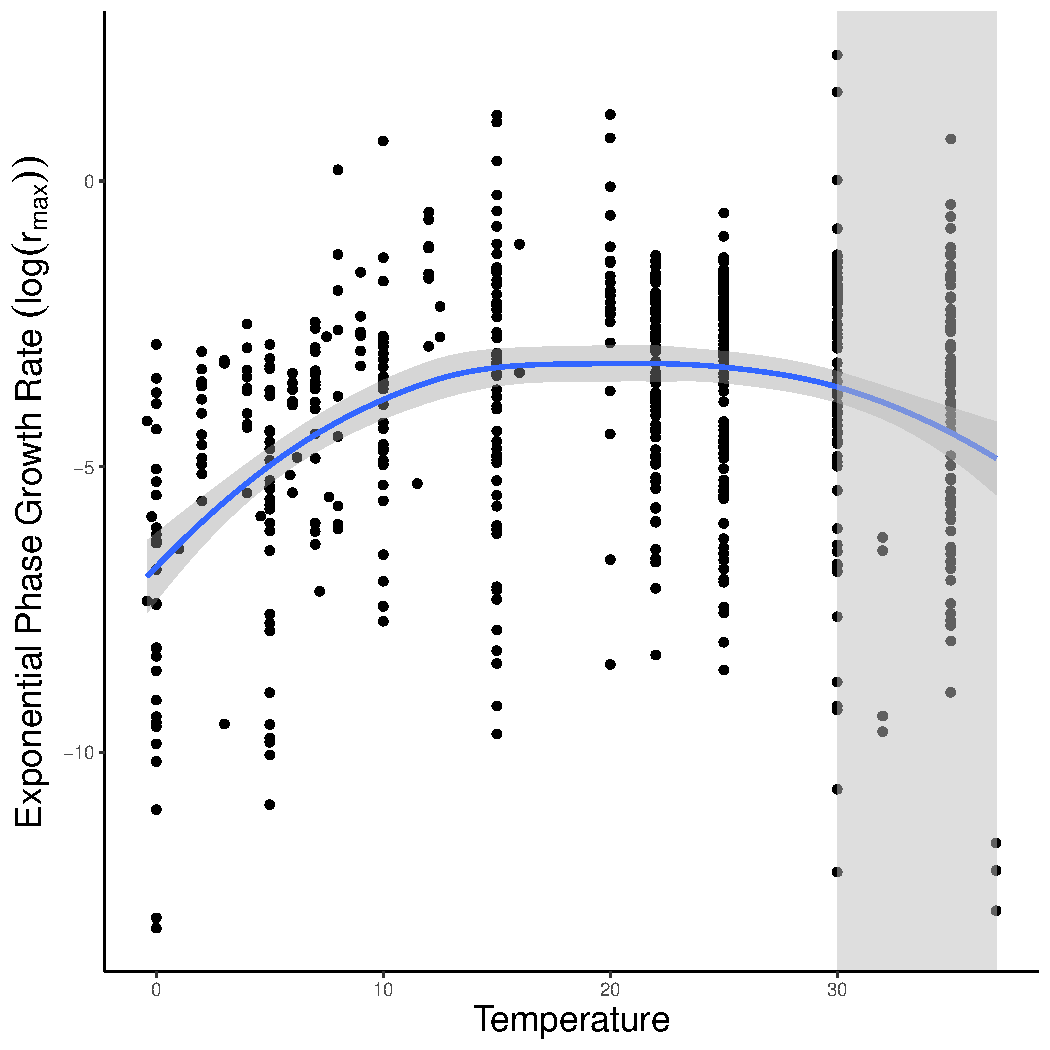
\includegraphics[width=.9\linewidth]{Plot/log_r_temp.pdf}
      \caption{}
      \label{fig:log_r_temp}
    \end{subfigure}%
    \begin{subfigure}{.47\textwidth}
      \centering
      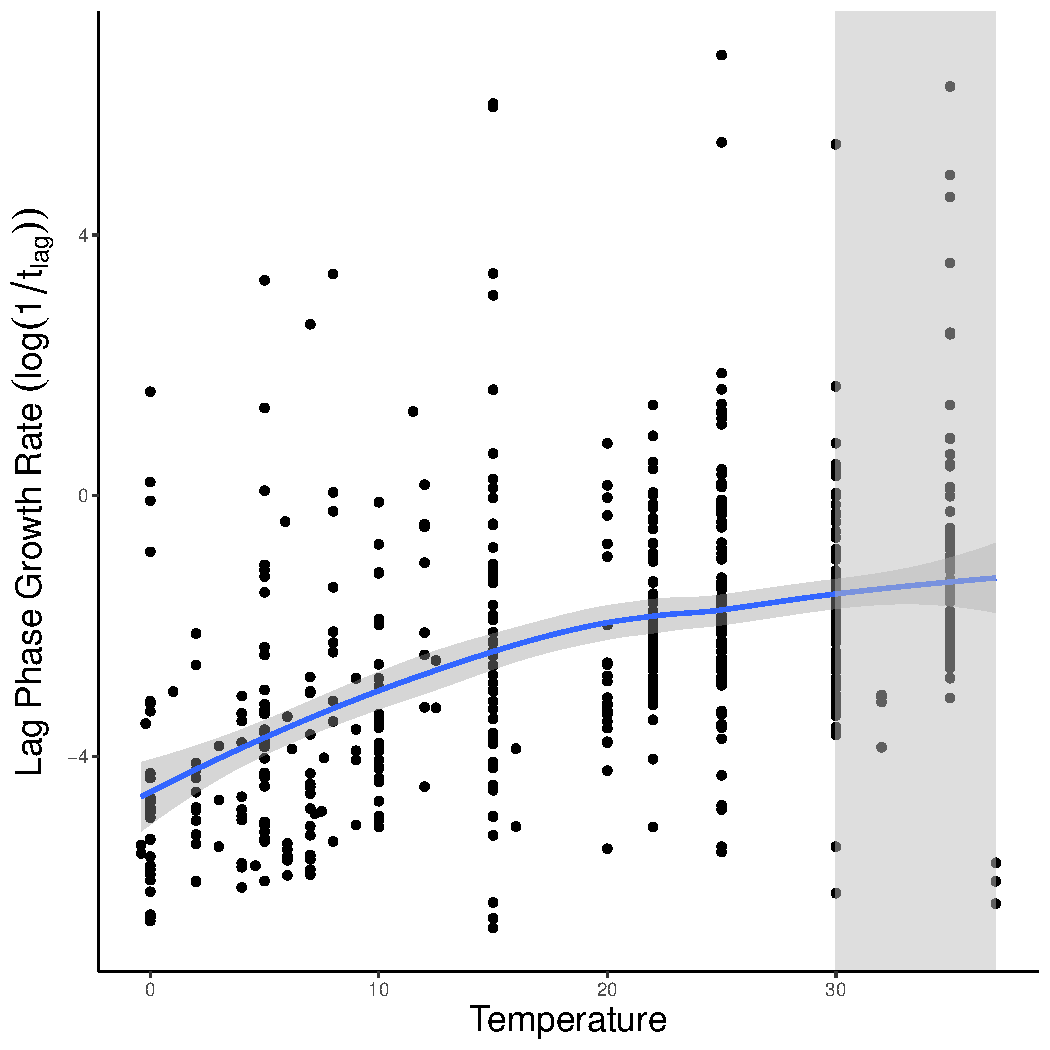
\includegraphics[width=.9\linewidth]{Plot/log_1tlag_temp.pdf}
      \caption{}
      \label{fig:log_1tlag_temp}
    \end{subfigure}
    \begin{subfigure}{.47\textwidth}
      \centering
      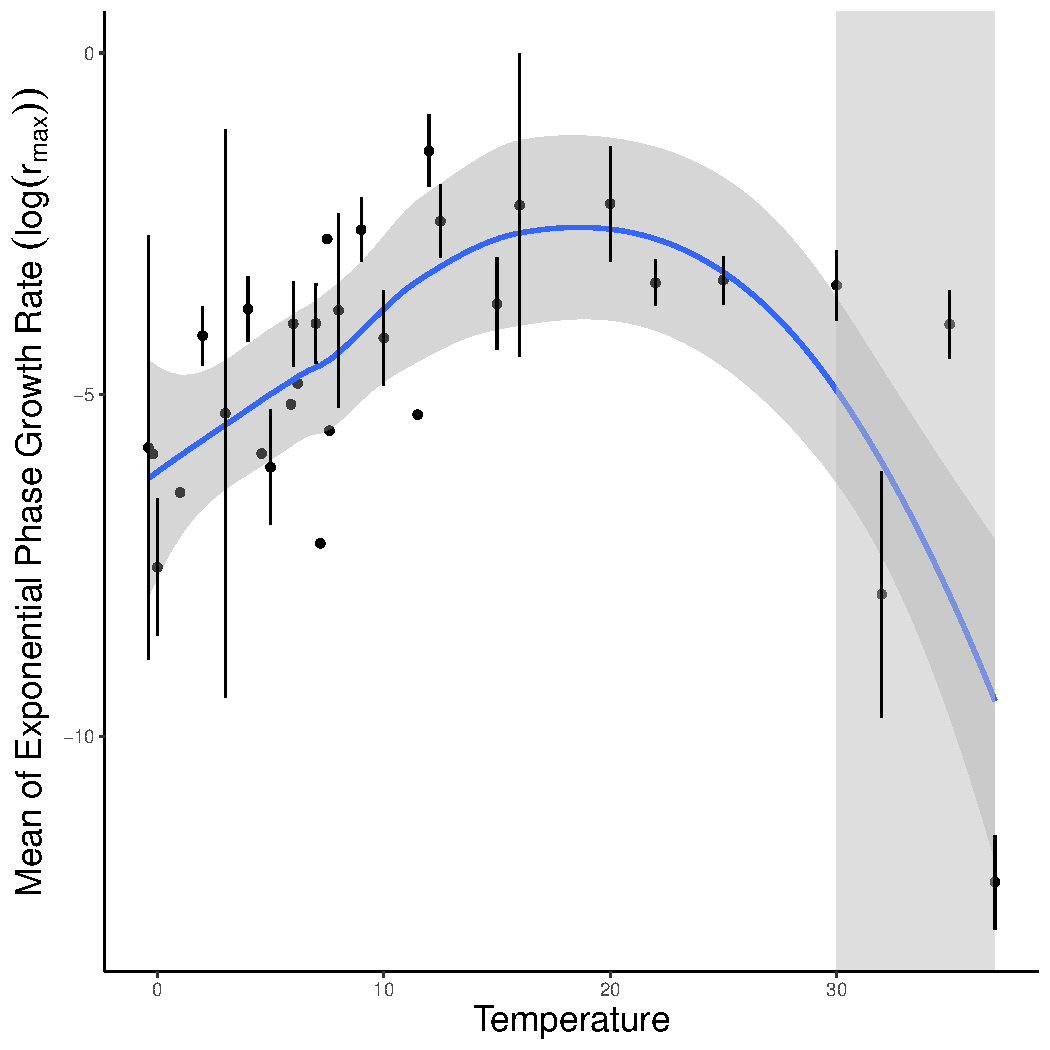
\includegraphics[width=.9\linewidth]{Plot/log_mean_r_temp.pdf}
      \caption{}
      \label{fig:log_mean_r_temp}
    \end{subfigure}%
    \begin{subfigure}{.47\textwidth}
      \centering
      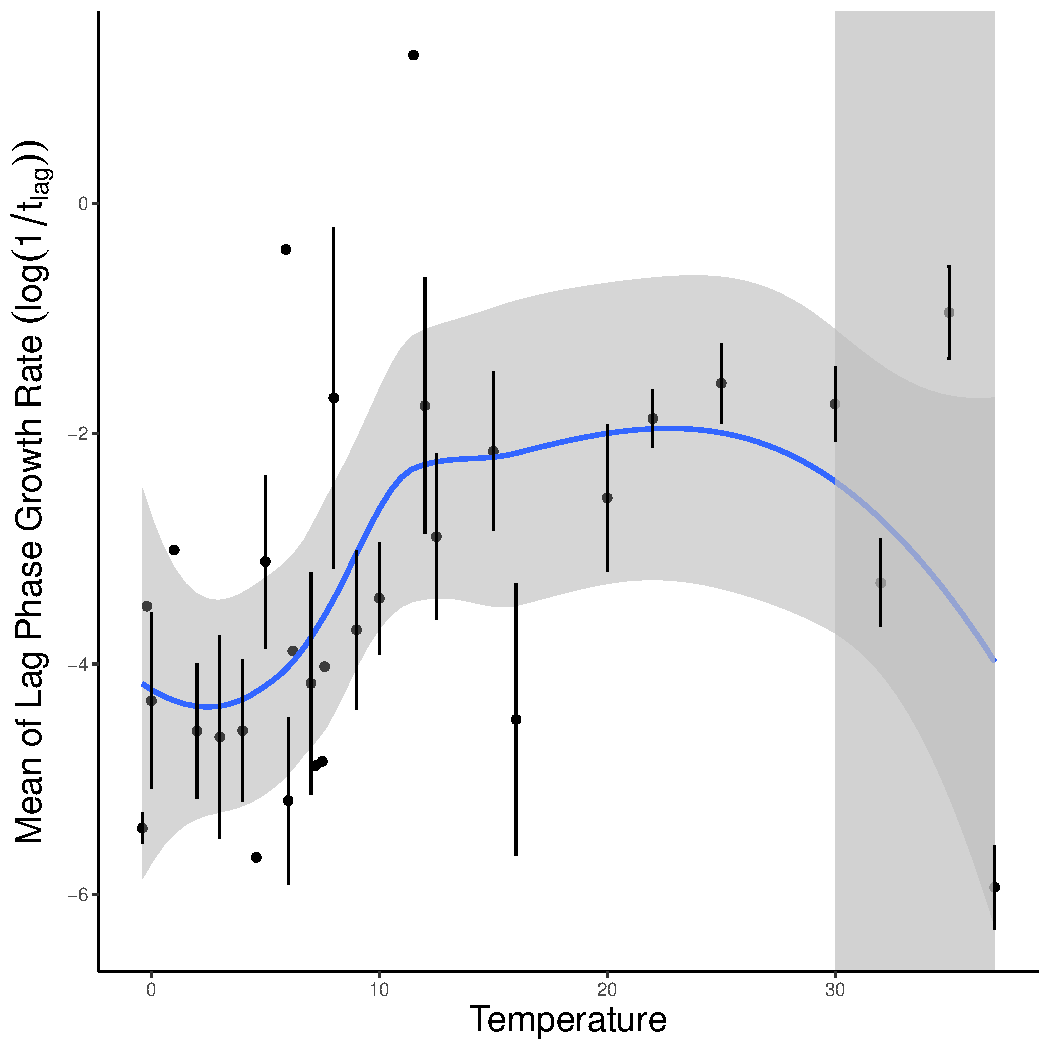
\includegraphics[width=.9\linewidth]{Plot/log_mean_1tlag_temp.pdf}
      \caption{}
      \label{fig:log_mean_1tlag_temp}
    \end{subfigure}
%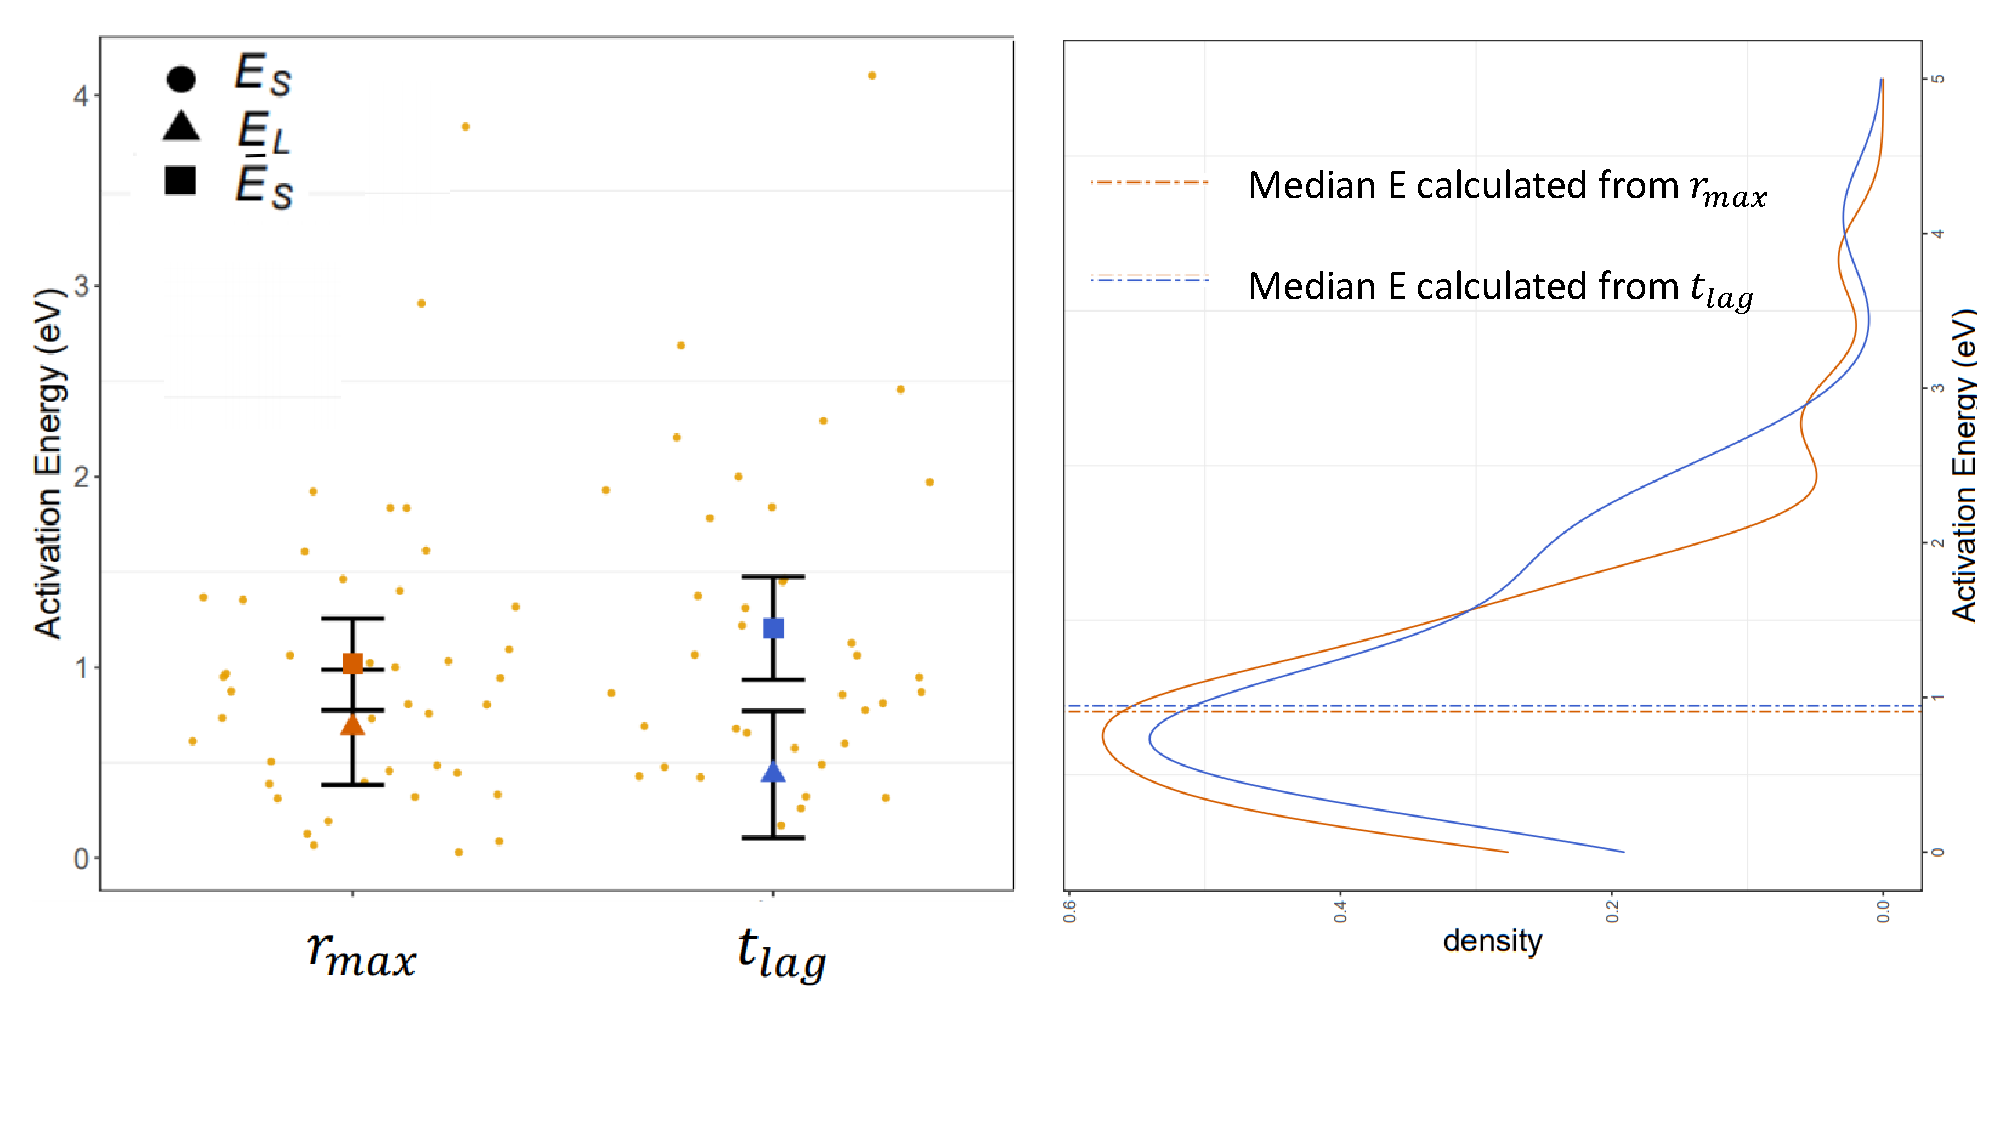
\includegraphics[width=1\linewidth]{Plot/E_comp.pdf}
\caption{Operational Temperature Range}\label{fig:rate_temp}
\flushleft{\normalsize General plot the trending of the temperature-dependent metabolic rate parameters. \textbf{a, c} are calculated from $r_{max}$, \textbf{b, d} are from $t_{lag}$. The curve regression line is fitted using 'loess' method in ggplot2 package with 95\% confidence interval. The plot \textbf{c, d} show the mean metabolic rate values. Error bars represent 95\% confidence interval calculated from normal distribution. By roughly scanning the trend, 30$^{\circ}$C is taken as Operational Temperature Range upper bound.}
\end{figure}
%, and the data points with temperature value higher than 30$^{\circ}$C would be discarded in the latter analysis.\\


% 3
\subsection{Thermal Response Comparison}

For both growth phases, the $\bar{E}_{S} > E_L > 0$ (Fig. \ref{fig:E_comp}, table \ref{table:E_mean}), follows the pattern in \textbf{c} of Fig. \ref{fig:E_short_long_cite}. As explained in Fig. \ref{fig:E_short_long_cite} about inferring the strength of the thermodynamic constraints on ectotherms. My result shows the thermal sensitivities are partially constrained by thermodynamic. In other words, selection does not completely override thermodynamic constraints, but there is some biochemical adaptation. Further detail about the activation energy of each species can be found in the supplementary information (Fig. \ref{fig:E_Spe}, table \ref{table:E_rmax_table} and table \ref{table:E_tlag_table}). \\

\begin{center}

\begin{table}[ht]
\centering
\begin{tabular}{lllll}
  \hline
  Time Scale & $E_{r_{max}}(eV)$ & $N_{rmax}$ & $E_{t_{lag}}(eV)$ & $N_{tlag}$ \\ 
  \hline
  short term & 1.02 $\pm$ 0.24 & 42 & 1.20 $\pm$ 0.27 & 37 \\ 
  long term &  0.68 $\pm$ 0.30 & 93 & 0.44 $\pm$ 0.33 & 90 \\ 
  \hline
\end{tabular}

% add caption and label
\caption{Two Phases short-/long-trem Activation Energy Comparison}
{\footnotesize Comparison of short-term and long-term activation energy values calculated from lag phases and exponential growth phase $\pm$ 95\% confidence interval. Data size is denoted by N}
\label{table:E_mean}

\end{table}





\end{center}
\begin{figure}[ht!]
\centering
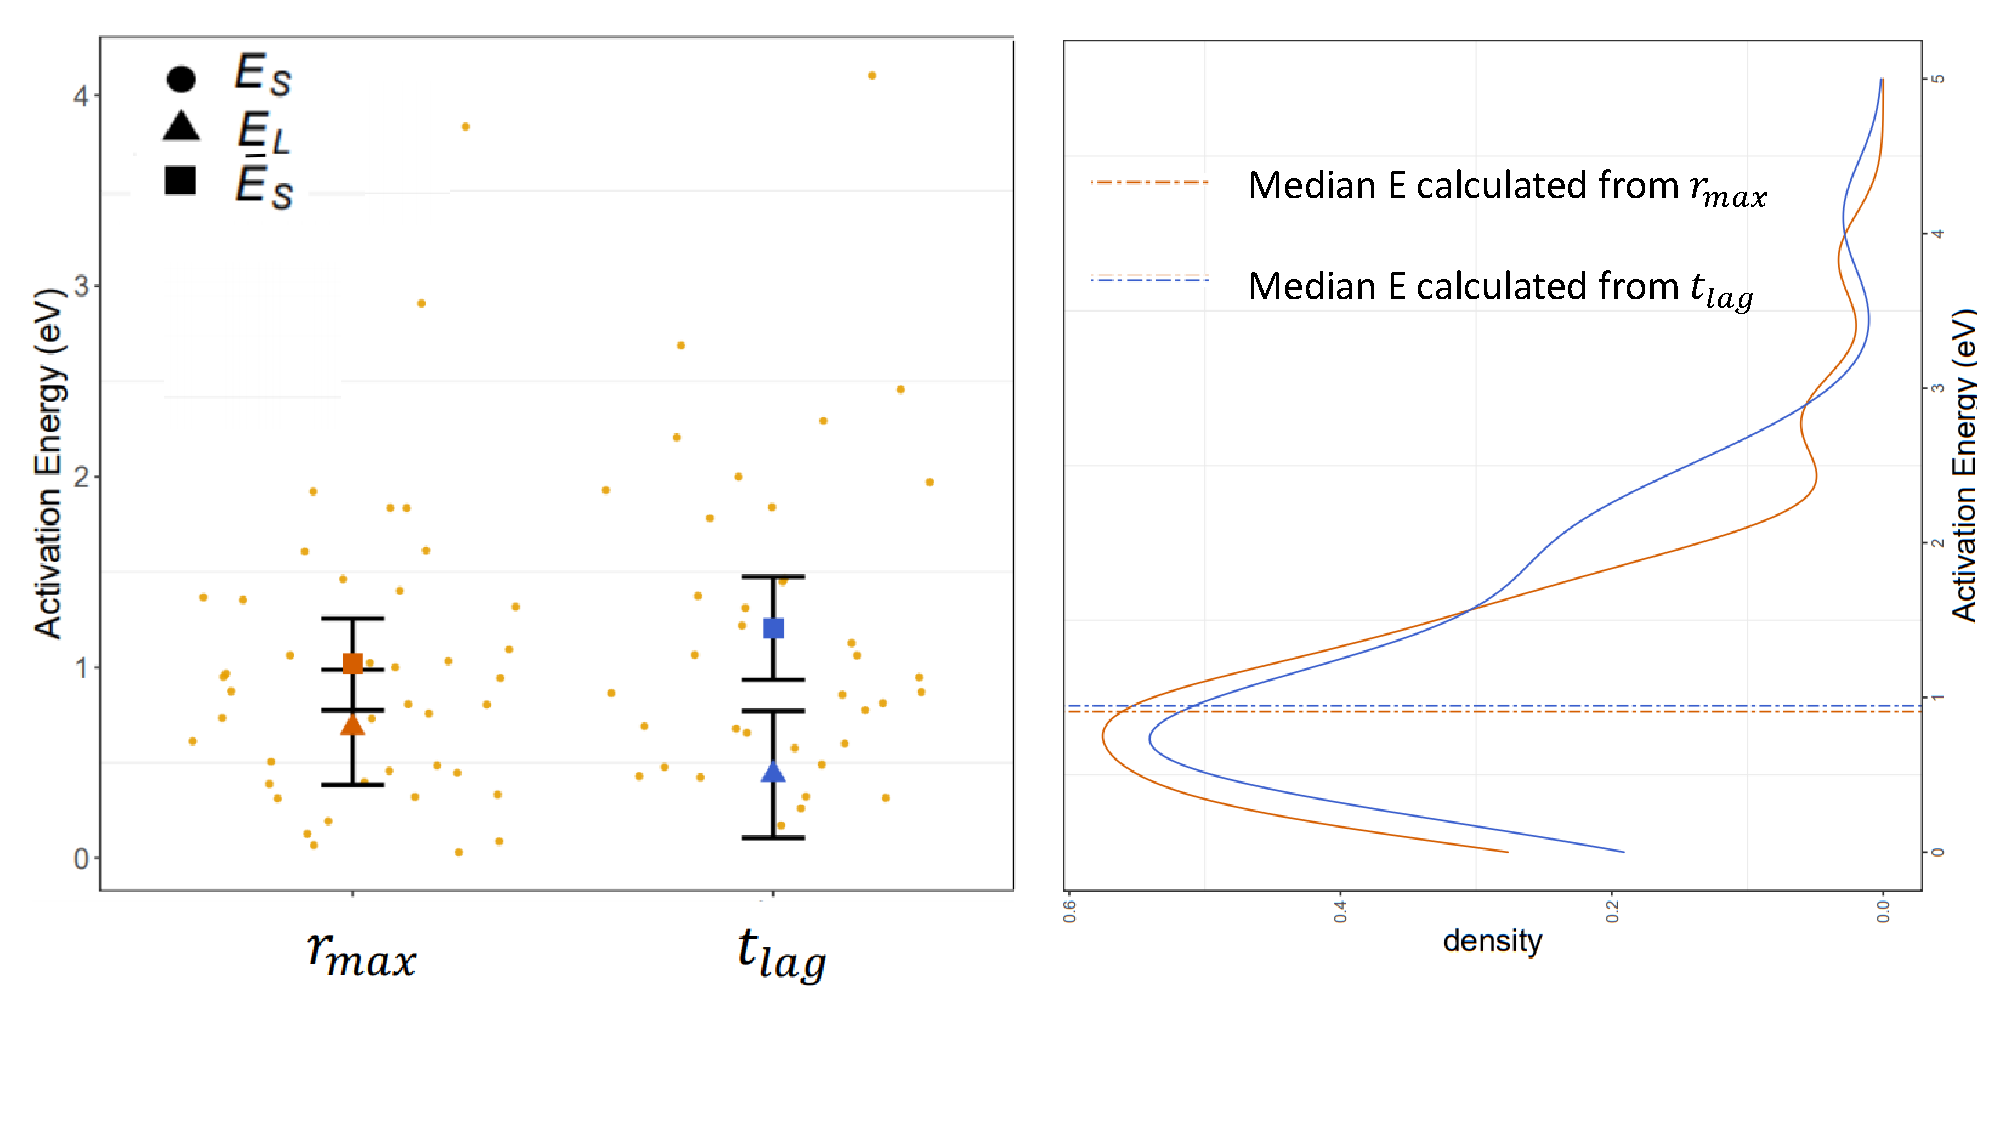
\includegraphics[width=1\linewidth]{Plot/E_comp.pdf}
\caption{Activation Energy Comparison}\label{fig:E_comp}
\flushleft{\normalsize \textbf{a} The thermal responses of each species ($E_S$, yellow dots). The mean value ($\bar{E}_{S}$, squares) of them is taken as the short-term thermal responses of exponential and lag phases. The long-term thermal responses ($E_L$, triangles) were calculated using the best performance metabolic rate parameters in each species. Both short-term and long-term thermal responses have error bars with 95\% confidence intervals. Orange symbols denote values calculated from exponential phase, blue ones denote lag phase. 
\textbf{b} Distribution of activation energy of species estimated from exponential (orange) and lag (blue) phases. The two "twodash" lines represent median activation energy values.
% , "dotted" lines represent mean activation energy value
}
\end{figure}

Moreover, if we take the difference between short-term and long-term activation energy ($\bar{E}_S - E_L$) estimated from metabolic traits as the degree of adaptation. In my result, estimating this measurement from parameter $1/t_{lag}$ is higher than from $r_{max}$ means the intensity of adaptation is stronger observed in the lag phase. \\

%From that we can infer there is acclimation during lag to exponential phase. Especially, if you consider the higher activation energy as stronger thermal sensitivity (less adapt to climate change), the short-term thermal response in exponential phase($\bar{E}_{S_{(r_{max})}}$) is higher than in lag phase($\bar{E}_{S_{(t_{lag})}}$), but the long-term thermal response in exponential phase($E_{L_{(r_{max})}}$) is even lower than in lag phase($E_{L_{(t_{lag})}}$) shows much acclimation ability in exponential phase. Further, by visually compare the $\bar{E}_{S}$ values estimated from exponential and lag phase, they are not significantly different, combined with the analysis above, it could tell that most of the acclimation appears in the exponential growth phase, it could also say that lag phase is more sensitive to temperature. \\



%%%%%%%%%%%%%%%%%%%%%%%%%% Discussion %%%%%%%%%%%%%%%%%%%%%%%%%% 
\section{Discussion}

% retreat from the beginning
This study examined the thermal response of two key metabolic traits (duration of lag phase and exponential growth rate) of microbes within and across species. I find stronger evidence for adaptation of the lag phase compared to the exponential phase. As under same constant experimental conditions, the stronger ability to suppress the thermodynamic constrain in lag phase could be achieved by the underlying metabolic mechanism of microbes. It got me to think that if this adaptation is autonomous, it is likely a response to selection for the ability of microorganisms to allocate limiting resources adjusting to the better metabolic rate in coping with constantly changing environmental conditions, such as different temperatures. \\

%The first result of a positive correlation between the two metabolic traits (Fig. \ref{fig:log_rt_col_temp}), agrees with recent work \citep{de2018determination}. While it is also compared in various specific conditions that each metabolic traits are estimated from the data sets with same environmental conditions. Further analysis calculating activation energy will let us see the general underlying patterns of microbial thermodynamic responses in exponential and lag growth phases. \\ 

The result that the short-term thermal sensitivity is higher in the lag phase than in exponential phase is contradicts to the results of \citealt{de2018determination},  who found that $r_{max}$ has the higher short-term thermal sensitivity (table \ref{table:E_comp_table}). The predicted activation energy values from two metabolic traits in this study were both relatively higher than those found by previous works \citealt{de2018determination} and \citealt{smith2019community}. This could be because I used \texttt{lm()} function in R to fit the Boltzmann-Arrhenius model, it may probably happen to use the steepest curve of the Temperature Performance Curve so got the higher value. Despite this potential limitation my result comparing the activation energy from both exponential and lag phases would not be affected, because the comparison is under the same temperature range. Further work could use the Sharpe–Schoolfield model \citep{shi2010comparison} as an alternative to Boltzmann–Arrhenius model. It would obtain a more precise Operational Temperature Range below the highest metabolic traits. So that the activation energy values may not as higher as in my study, it may lead to different result in further research. \\
\begin{center}

\begin{table}[ht]
\centering
\begin{tabular}{lll}
  \hline
  Reference & $E_{r_{max}}(eV)$ & $E_{t_{lag}}(eV)$  \\ 
  \hline
  current study & 1.02 $\pm$ 0.24 & 1.20 $\pm$ 0.27 \\
  \citep{de2018determination} & 0.95 & 0.83 \\ 
  \citep{smith2019community} & 0.87 $\pm$ 0.05 & None \\
  \hline
\end{tabular}
% \diagbox{Time}{Day}

% add caption and label
\caption{Activation Energy Comparison with Previous Works}
{\footnotesize Comparison of short-term activation energy values calculated from the lag phase and the exponential growth phase in the current study and in previous work \citep{de2018determination,smith2019community}}
\label{table:E_comp_table}

\end{table}

\end{center}


%\subsection{Diauxic Growth Pattern}
Multi carbon substrate supply is another widely concerning environmental factor that could cause the lag phase in the microbial growth curve. Facing several carbon resources, the microbes switch hierarchically between them from the most favourite to the least, leading to biphasic growth curves also called diauxic growth \citep{monod1949growth}. During these diauxic phases, the microbes could be vulnerable to harsh perturbations such as heat, as they are undergoing processes adjusting to the new environment. Could the duration of the lag phase be a stress indicator \citep{hamill2020microbial}? Understanding the underlying mechanism of microbes' special sensitivity to temperature change could make them the eco-friendly guide organisms used to monitor environmental change. \\
%and maintain the ecosystems function. \\
% Most of the works in this field focus on the underlying molecular regulations and the the well-known phenomenon -- the crabtree effect: glucose-induced repression of genes involved in the uptake and metabolism of alternative carbohydrates \citep{perez2018crabtree}. The study of the general metabolic pattern can also further the understanding of such field. \\

% \subsection{Short-term and Long-term Comparison}
My result that the difference of activation energy calculated from the lag phase is higher than from the exponential phase suggests that there is more adaptation in the lag phase. In other words, it is less restricted by thermodynamics. Following the approach of \citealt{hamill2020microbial}, further research could also investigate whether the reduced thermal restriction or also higher degree of adaptability of the lag phase, could be an indication of stronger competitive ability. Furthermore, as the lag phase is the initial growth phase that microbes enter, the metabolic strategies they employ could have a profound influence on their competitiveness in later life cycles. \\

% \subsection{Dynamic Interaction}
If we want to analyse the competitive ability of species from the perspective of thermal response patterns of metabolic traits, the trait values estimated in my study alone are not enough. Because in my research, the fitness of the population is assessed independently of other perturbations or interactions in the systems, which is a less perfect reflection of what really happens in the real world. In the real world, microbial populations mostly exists as a component of communities interacting with other species and influenced by environmental conditions. If we want to understand the broader microbial communities, we need to understand those interactions incorporating microbial community structures, dynamics, functions and networks etc. \\

For obtaining more reliable predictions of competitiveness, a more precise determination of the fitness of a genotype is required. The in-silico simulation could be an ideal way to achieve this. For example, a recent study has constructed an approach to predict relative density-dependent fitness accounting for the effects of each growth cycle on fitness \citep{ram2019predicting}. This research took culture medium as a variable, a similar future work could be constructed to predict relative fitness based on thermal response. \\

Models incorporating species interactions and environmental perturbations can also be found in recent studies \citep{rodrigues2021community, pacciani2020dynamic, li2020modeling}. \citealt{rodrigues2021community} considered resource competition. They incorporated demographic composition and found that cooperative behaviour in the early and late life span are both not favoured. They also found that niche expansion can promote mutualism. \citealt{pacciani2020dynamic} studied dynamic metabolic adaptation as a mechanism to maintain biodiversity. Incorporating thermal constraints in their model could make it more useful in practical applications. While \citealt{pacciani2020dynamic} just assign the metabolic rate value in the model, \citep{li2020modeling} built a model that makes it dynamic, mapping from metabolic strategies to fitness consequences. Their model is based on resource-competition models using the adaptive dynamic technique, but in contrast to the adaptive dynamic technique, it takes the metabolic rate as dynamic. In their study, \citealt{li2020modeling} found the dynamic fitness landscape is changing with species-environment feedback. On that basis, \citealt{li2020modeling} studied how could the microbes allocate the resource to maintain the most fitness metabolic behaviour. Further research similar to \citealt{li2020modeling} could incorporate temperature as a critical factor influencing metabolic strategies. \\ % \citealt{li2020modeling} under the conditions of chemostat

% There are some short-comings of my analysis:  \subsection{Caveats}
My study has some limitations that could be addressed with future work. The calculation of short-term thermal responses $\bar{E}_{S_{rmax}}$ and $\bar{E}_{S_{tlag}}$ are simply the average of activation energy of each species. An alternative approach would be to cancel the bias from poor fitting data sets by taking the weighted average instead. The data sets in my study were collected for analysing the growth rate of the microbes, it is not guaranteed that each species strain contains a series of temperatures so that it can be used to examining the microbes' response to temperature. For this reason, in my study, many data sets were invalid. A larger data size (table \ref{table:E_mean}) may lead to a different result and could be more persuasive. And collecting experiment data use temperature as the independent variable is more suitable for this study.\\

% Conclusion
% Given the critical role of microorganisms in ecology, a wide range of applications come with it. 
In this study, by comparing the metabolic traits I found different degrees of adaptation in life cycles, which could lead to stronger competitiveness of microbes. While throughout the whole life cycle temperature takes a critical role in constraining biological rates, recent studies do not take this constrain into consideration. The results of this study deepen our understanding of thermodynamic constraints on metabolic traits, thus laying the foundation for understanding mechanisms underlying competition between microbial taxa across environmental gradients. \\


%Because in early stage the costs surpass the benefits and in late stage due to the resource depletion.  

% Further metabolic allocation research is needed to further this field for better understanding the competition and cooperation strategies of microbes. also studied if the nutrient niche is expanded by cross-feeding or other mechanisms, will it lead the 


% interaction: The model constructed by \citep{rodrigues2021community} by considering the species competing for the same resource by cooperate in the mean time through niche expansion. we can also study how the temperature fluctuation influence the interactions between species. \\
%In study \citep{rodrigues2021community} they found that the helping behaviour in the early and late life span are both not favoured. Because in early stage......they assume the carrying capacity is fixed. In such zero-sum game, competition of limiting resources which must take the fitness as dencity-dependent , could the early stage deficiency of providing help to relative species is constrained by the metabolic rate which is constrained by the thermodynamic? 
% \citep{rodrigues2021community} also the evolution of cooperation is influenced by the intrinsic growth rate of species compete for shared resources, it can neither be too slow to be surpassed by partner species, nor too high of exclude the relative species.  \\

% because the species would not behaving in my model as there is nothing else around them, nothing else is trying to competing for the same resources
%1. dynamic 
%2. competition
%Many previous work take the environment as static, simplified the work of natural selection as finding the maximum strategy on the stationary fitness landscape. The adaptive dynamic also known as evolutionary invasion analysis, provided a framework of addressing long-term evolution of traits taken the fitness as the density dependent. Although the adaptive dynamics models have already considered the interaction of other species, the environment is also constantly changing corresponding to the feadback from individuals in the community. Recent study \citep{li2020modeling} based on the idea of adaptive dynamics, measures the fitness of composition in the study system considering the specific environment conditions. The improvement of this model modified the measurement of the fitness not only is frequency dependent, which only consider the competition relationship but also incorporate the environmental influencing factors.
%3. cross-feeding






%Follow-up research should be designed for collecting data for the problem purposefully. \\

%to  may lead to different estimated short-term activation energy values, so could be the later difference comparison. \\
%The possible limitations of my study include that as For the activation energy difference between the short-term ($\bar{E}_S$) and long-term ($E_L$) comparison in this study, there is one thing that needs attention that just calculated by simply took the average of the activation energy of each species $E_S$. 

% 3. The data size is not large enough may lead to some deviation. Also, the data sets are collected , it is not   

% The Boltzmann-Arrhenius model was fitted just using the \texttt{lm()} function in R, witch could be just taken as the rough fitting. To improve the presision of the fitting, I would choose fitting the Sharpe–Schoolfield model as an alternative to Boltzmann–Arrhenius 1. why \citep{smith2019community} use the Sharpe–Schoolfield model as an alternative to Boltzmann–Arrhenius? what does it mean it may be an interesting approach to predicting the effects of extreme warming events at the ecosystem level? However, parameterising this would again require the data on the specific species present in a given ecosystem and their individual TPCs, which is outside of the scope of our current study.% the result could be more precise and more persuasive. it could be not precise so will influence .  \\

% Most microbial systems in nature as the open systems are constituted in high dynamic community.  

% not only get more diverse influence from out side world, it is in need for incorporating the peer's makeup and considering the interactions between them, for instance, the most commonly studied competition or cooperation effects. \\

% community net work, functions, dynamics, microbial community structure\\

% For gaining implications of the short- and long-term thermal responses of microbes for ecosystem functioning, testing activation energies of underlying metabolic flux rates is necessary. Similar analyses has been implemented by \citep{smith2019community}.

%\citep{new2014different} 

%carbon catabolite repression (CCR) \citep{gorke2008carbon}\\

% MTE provides an approeche incorparatting the first laws of physics and chemistry of explaining the variation of the growth rate of the individuals, but it is clear the complex biological system can not just be explained just by temperature and body size, so other factors can be incorporate to test through simulation, thanks to the growing arithmetic speed. And recently there are already some studies has offered some conjecture and testing. For instance, \citep{perez2018crabtree} has reveled that the duration of the lag phase is limited by respiratory energy conversion.\\

% How much can microbes adjust to different phase, optimizing it's potential to widen the thermal niche width \citep{kontopoulos2020phytoplankton} or maximize the biochemical reaction rate?\\



%%%%%%%%%%%%%%%%%%%%%% Data and Code Availability %%%%%%%%%%%%%%%%%%%%%%
\newpage
\section*{Data and Code Availability}
\addcontentsline{toc}{section}{Data and Code Availability}
All the code for replicate this dissertation can be found in the \href{https://github.com/zongyi2020/CMEEProject}{github repository}: \url{https://github.com/zongyi2020/CMEEProject}

%%%%%%%%%%%%%%%%%%%%%%  Acknowledgements %%%%%%%%%%%%%%%%%%%%%% 
\newpage
\section*{Acknowledgements}
\addcontentsline{toc}{section}{Acknowledgement}

Throughout process of my dissertation I have received a great deal of support and assistance from my supervisors. I would like to thank my supervisors, Dr. Samraat Pawar, Dr. James Rosindell and Dr. David Orme, whose guidance was invaluable in inspiring me exploring deeper in to area of expertise. Your insightful feedback leaded me to widen my thought and brought my work to efficiency.

% I would like to acknowledge my colleagues from my internship at Central P. for their wonderful collaboration. I would particularly like to single out my supervisor at Central P., Phoebe Buffay. Phoebe, I want to thank you for your patient support and for all of the opportunities I was given to further my research.

% I would also like to thank my tutors, Dr. Ross Geller and Dr. Chandler Bing, for their valuable guidance throughout my studies. You provided me with the tools that I needed to choose the right direction and successfully complete my dissertation.

In addition, I would like to thank my parents for their wise counsel and support. You are always there for me. % Finally, I could not have completed this dissertation without the support of my friends, Joey Tribbiani and Rachel Green, who provided stimulating discussions as well as happy distractions to rest my mind outside of my research.


%%%%%%%%%%%%%%%%%%%%%% bibliography %%%%%%%%%%%%%%%%%%%%%%
\clearpage
\bibliographystyle{agsm}
\bibliography{bib}

%%%%%%%%%%%%%%%%%%%%%% appendix %%%%%%%%%%%%%%%%%%%%%%
\newpage
\appendix
\section{Supplementary Information}

\subsection{Data} \label{Data_SI}
\citep{bae2014growth,blagodatskaya2007priming,galarz2016predicting,gill1991growth,heo2009estimation,inoue1977effect,kapetanakou2019model,kirchman1997regulation,koutsoumanis2006development,lee2007model,phillips1987relation,roth1962continuity,silva2018modelling,sivonen1990effects,stannard1985temperature,vankerschaver1996influence,willocx1993modelling,zwietering1994modeling}

%%% problematic citation if adding in bib file
% \citep{bernhardt2018metabolic}




%%%%%% Operational Temperature Range
% \newpage
\subsection{Operational Temperature Range}

\begin{figure}[htb]
\centering
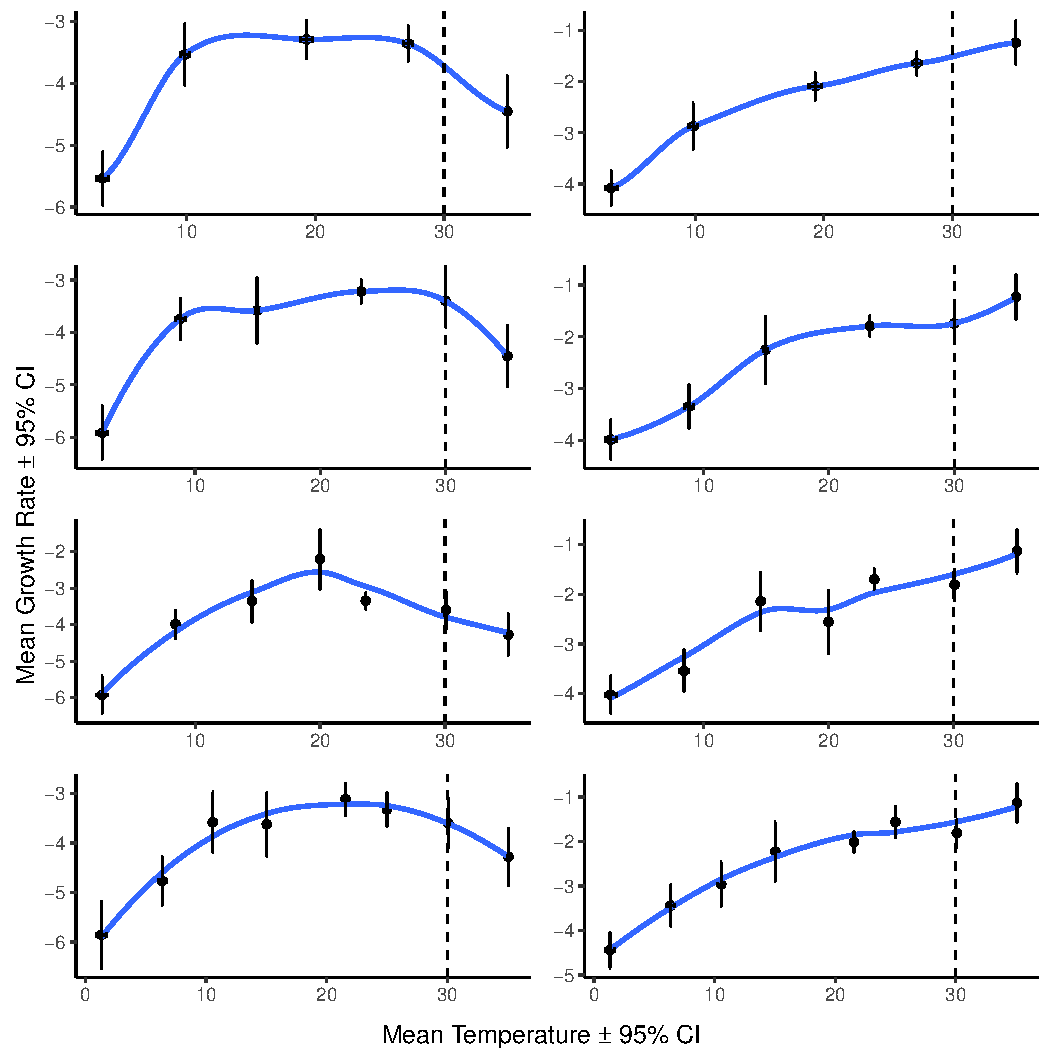
\includegraphics[width=1\textwidth]{Plot/mean_rate_temp_group.pdf}
\caption{Operational Temperature Range Grouped by Temperature}\label{fig:mean_rate_temp_group}
{\footnotesize Across species mean maximum growth rate ($log(r_{max})$, left) and lag phase growth rate ($log(1/t_{lag})$, right) with 95\% confidence interval in different groups of temperature, from the first to the forth row represents 5-8 groups respectively.}
\end{figure}



%%%%%%%%%%%
\subsection{Typical Model Fitting Plot}
\begin{figure}[ht!]
\centering
    \begin{subfigure}{.47\textwidth}
      \centering
      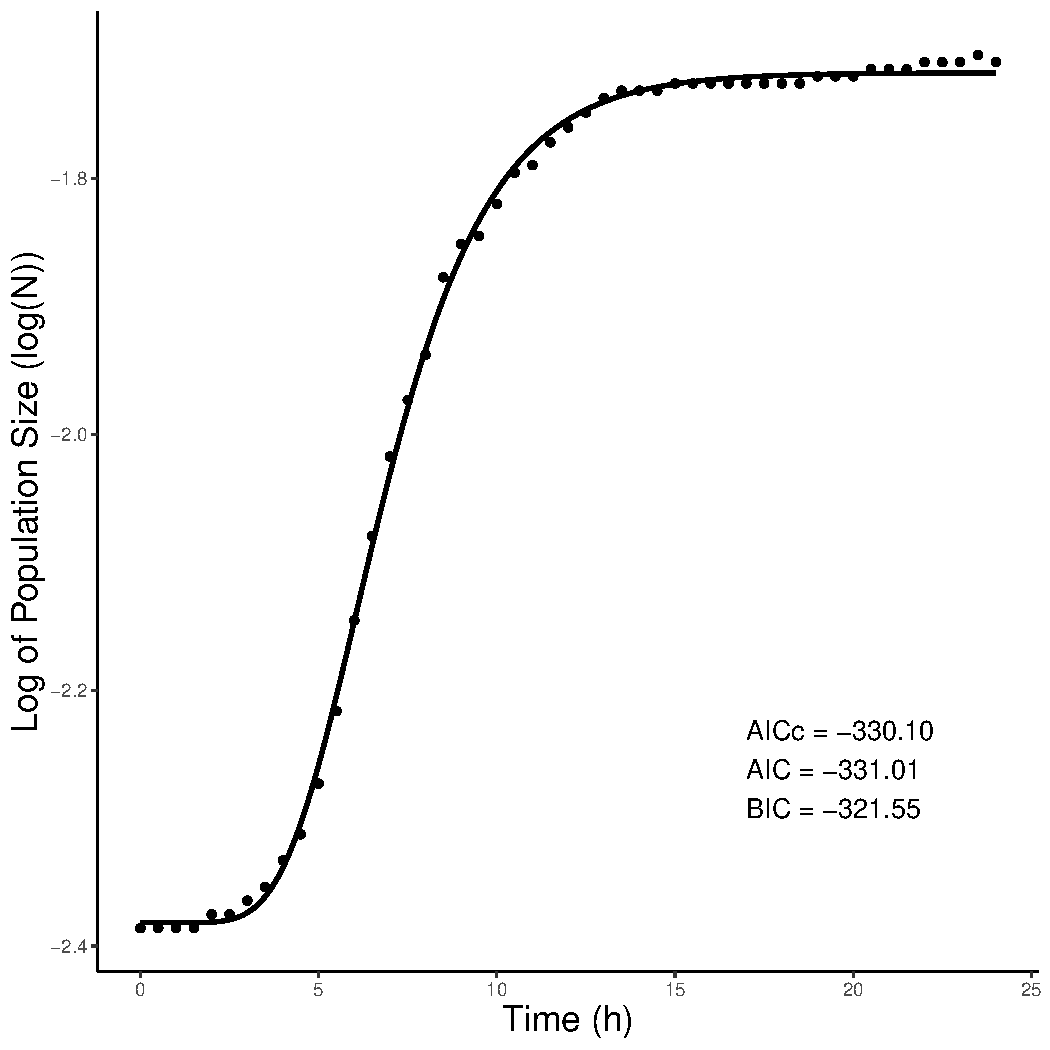
\includegraphics[width=.9\linewidth]{Plot/typ_gomp_fit.pdf}
      \caption{Typical Gompertz Model Fitting Plot}
      \label{fig:typ_gomp_fit}
    \end{subfigure}%
    \begin{subfigure}{.47\textwidth}
      \centering
      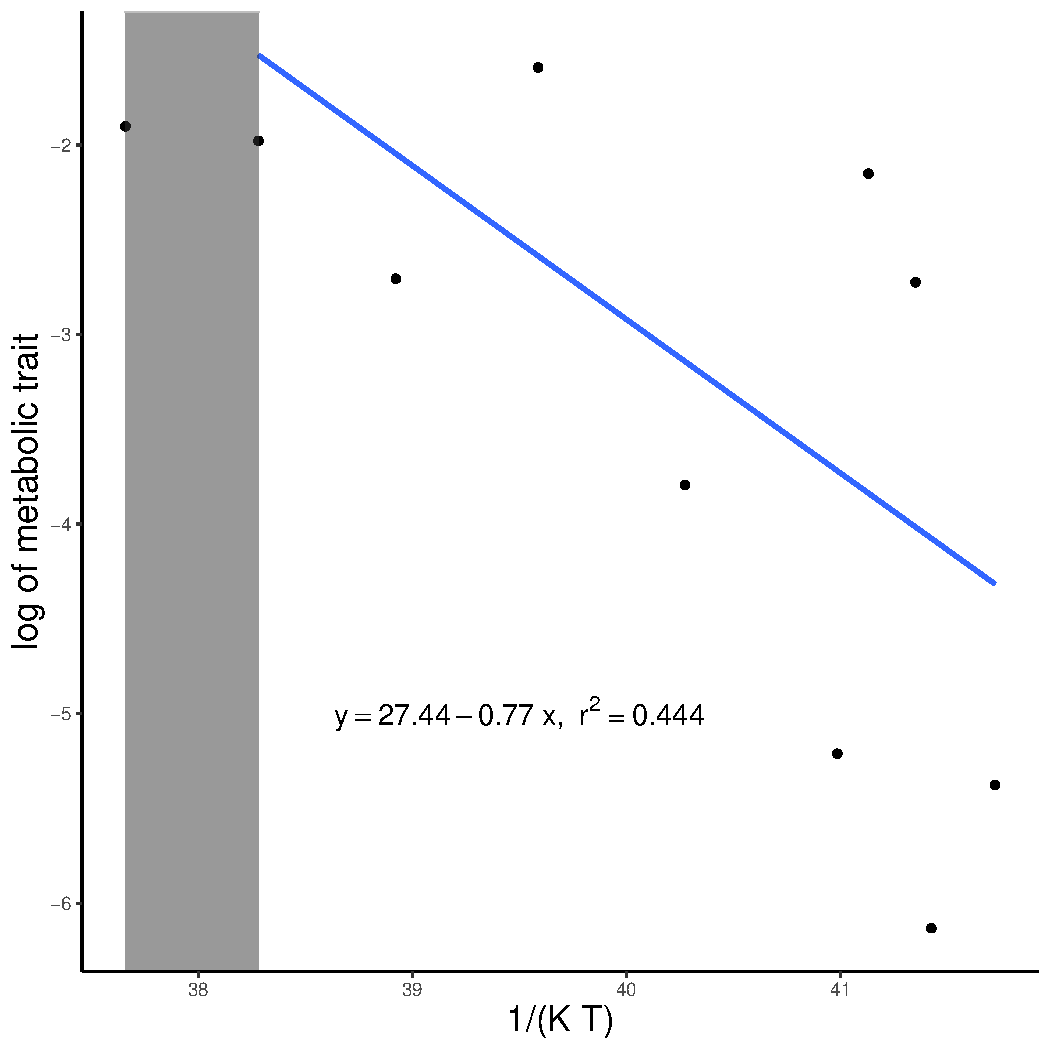
\includegraphics[width=.9\linewidth]{Plot/typ_arrhe_fit.pdf}
      \caption{Typical Boltzmann-Arrhenius Model Fitting Plot}
      \label{fig:typ_arrhe_fit}
    \end{subfigure}

\caption{Typical Model Fitting Plot}\label{fig:typ_fit}
{\footnotesize The typical model fitting plots. \textbf{a} A typical Gompertz Model fitting plot with \textit{AICc, AIC, BIC} as goodness of fit criteria. \textbf{b} A typical Boltzmann-Arrhenius model fitting plot with \textit{$r^2$}}
\end{figure}

%%% Activation Energy
%\newpage
\subsection{Activation Energy}

% figure
%1
\begin{figure}[ht!]
\centering
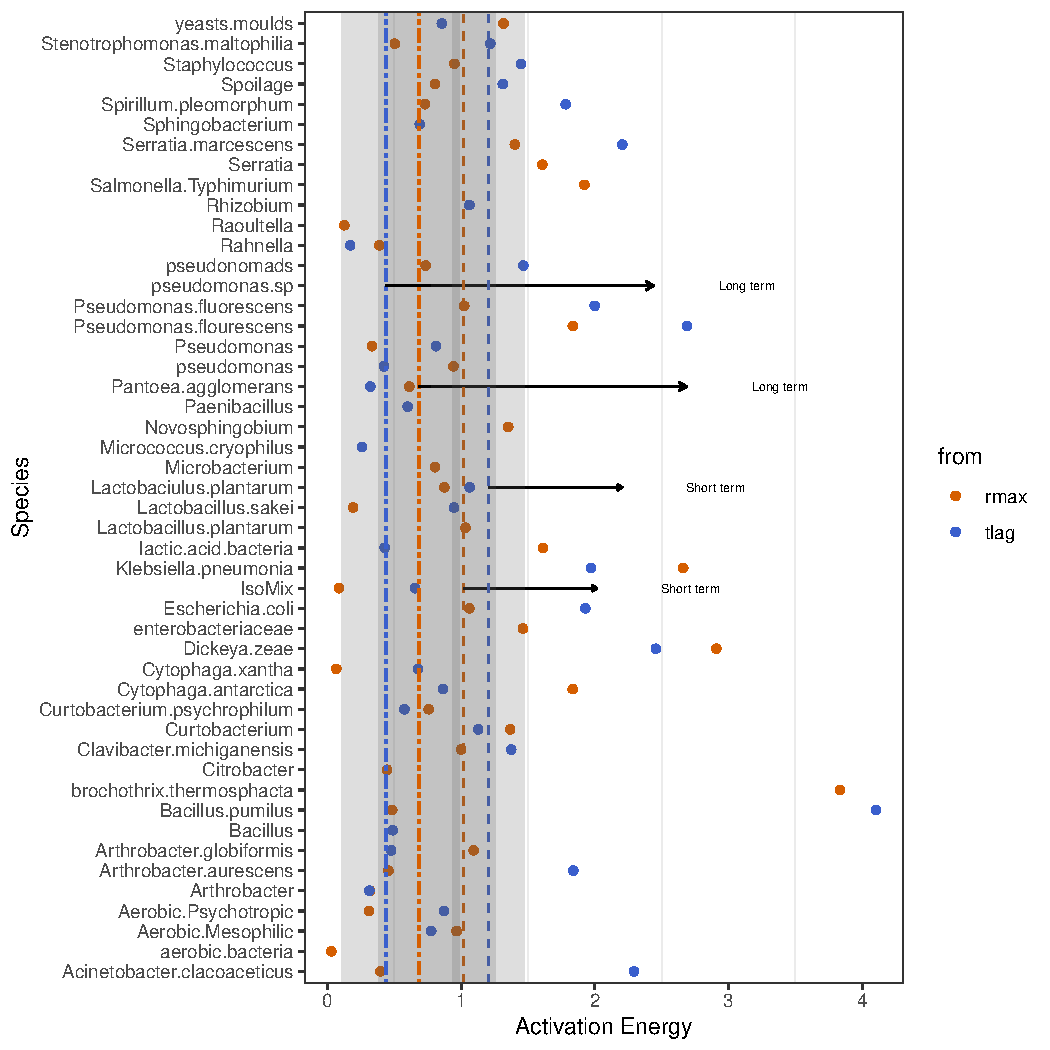
\includegraphics[width=1\linewidth]{Plot/E_spe.pdf}
\caption{Activation Energy of Each Species}\label{fig:E_Spe}
{\footnotesize Variation in short-term thermal sensitivity($E_S$) amongst bacteria groups, with vertical dash lines annotating the mean variations($\Bar{E}_S$, short-term) and the long-term($E_L$) sensitivity both with 95\% confidence interval}
\end{figure}

\begin{center}
% latex table generated in R 4.1.0 by xtable 1.8-4 package
% Sun Aug 15 16:55:43 2021
\begin{table}[ht]
\centering
\begin{tabular}{rlrrr}
  \hline
 & Species & E.value & Confidence.Interval & P.value \\ 
  \hline
1 & Pantoea.agglomerans & 1.1555603903E+00 & 6.2858792339E-01 & 7.8941604021E-03 \\ 
  2 & Clavibacter.michiganensis & 1.2012386963E+00 & 7.2035536371E-01 & 2.0662485300E-02 \\ 
  3 & Stenotrophomonas.maltophilia & 5.4567831439E-01 & 4.4863565962E-01 & 4.1034677993E-02 \\ 
  4 & Bacillus.pumilus & 8.5985176303E-01 & 4.9767234461E-01 & 2.5924118012E-02 \\ 
  5 & Aerobic.Psychotropic & 8.6533345980E-01 & 4.2059531790E-01 & 8.1098910112E-04 \\ 
  6 & Aerobic.Mesophilic & 1.2406834647E+00 & 5.3111010753E-01 & 2.5506125596E-04 \\ 
  7 & Pseudomonas.flourescens & 4.7617684816E+00 & 2.3400073431E+00 & 4.7499765766E-03 \\ 
  8 & pseudomonas & 2.1701790335E+00 & 9.1882632739E-01 & 1.7972884006E-02 \\ 
  9 & Serratia.marcescens & 1.7970209613E+00 & 1.1803257185E+00 & 1.8715688310E-02 \\ 
  10 & Weissella.viridescens & 1.2285562277E+00 & 4.8211259590E-01 & 6.9993952483E-03 \\ 
  11 & Mean Value & 1.5825870793E+00 & 7.5005254309E-01 & 1.4501943621E-02 \\ 
   \hline
\end{tabular}
\end{table}

\end{center}
\begin{center}
% latex table generated in R 4.1.1 by xtable 1.8-4 package
% Sun Aug 22 20:00:15 2021
\begin{table}[ht]
\centering
\begin{tabular}{rlrr}
  \hline
 & Species & E.value & Confidence.Interval \\ 
  \hline
1 & Pantoea.agglomerans & 3.2065484995E-01 & 2.0261744474E+00 \\ 
  2 & Clavibacter.michiganensis & 1.3741532959E+00 & 2.7386069317E+00 \\ 
  3 & Stenotrophomonas.maltophilia & 1.2185292311E+00 & 5.7080248684E-01 \\ 
  4 & Klebsiella.pneumonia & 1.9716850572E+00 & 2.3071507342E+00 \\ 
  5 & Dickeya.zeae & 2.4560490952E+00 & 1.3909428718E+00 \\ 
  6 & Acinetobacter.clacoaceticus & 2.2927193394E+00 & 1.6426021111E+00 \\ 
  7 & Bacillus.pumilus & 4.1038884743E+00 & 2.7852972220E+00 \\ 
  8 & Pseudomonas.fluorescens & 1.9986844721E+00 & 4.5923828736E+00 \\ 
  9 & Staphylococcus & 1.4477321739E+00 & 4.6199587467E-01 \\ 
  10 & Pseudomonas & 8.1156355755E-01 & 2.7860276756E-01 \\ 
  11 & Aerobic.Psychotropic & 8.7054572161E-01 & 4.6369045704E-01 \\ 
  12 & Aerobic.Mesophilic & 7.7598733247E-01 & 5.7124030388E-01 \\ 
  13 & Spoilage & 1.3103794439E+00 & 1.5980454729E+00 \\ 
  14 & Escherichia.coli & 1.9290472286E+00 & 3.9536563108E+00 \\ 
  15 & Curtobacterium.psychrophilum & 5.7547281206E-01 & 8.2534829665E-01 \\ 
  16 & Cytophaga.antarctica & 8.6434179183E-01 & 5.6319675635E-01 \\ 
  17 & Cytophaga.xantha & 6.7703430495E-01 & 8.1564499817E-01 \\ 
  18 & Spirillum.pleomorphum & 1.7815692937E+00 & 8.7011892340E-01 \\ 
  19 & Micrococcus.cryophilus & 2.5849023891E-01 & 1.0705993267E+00 \\ 
  20 & Pseudomonas.flourescens & 2.6879164913E+00 & 2.7824753536E+00 \\ 
  21 & pseudomonas & 4.2227309562E-01 & 1.2827742161E+00 \\ 
  22 & yeasts.moulds & 8.5506851885E-01 & 1.6072729184E+00 \\ 
  23 & lactic.acid.bacteria & 4.2770108072E-01 & 2.5827988171E+00 \\ 
  24 & pseudonomads & 1.4648694644E+00 & 1.4386373967E+00 \\ 
  25 & Serratia.marcescens & 2.2052486393E+00 & 1.2403294563E+00 \\ 
  26 & Arthrobacter & 3.1328343052E-01 & 5.8346638330E-01 \\ 
  27 & Arthrobacter.aurescens & 1.8386360620E+00 & 1.7373564498E-01 \\ 
  28 & Arthrobacter.globiformis & 4.7629968860E-01 & 1.4098413475E+00 \\ 
  29 & Lactobacillus.sakei & 9.4621117146E-01 & 1.0086183868E+00 \\ 
  30 & Lactobaciulus.plantarum & 1.0642098106E+00 & 6.2787266075E-01 \\ 
  31 & Rahnella & 1.6967053479E-01 & 7.9940640337E-01 \\ 
  32 & Sphingobacterium & 6.9031618237E-01 & 1.7921975981E+00 \\ 
  33 & Rhizobium & 1.0610503552E+00 & 9.5983883501E-01 \\ 
  34 & Curtobacterium & 1.1268698833E+00 & 1.3894959862E+00 \\ 
  35 & IsoMix & 6.5587897228E-01 & 6.0147066300E-01 \\ 
  36 & Paenibacillus & 5.9979189848E-01 & 1.1831431247E+00 \\ 
  37 & Bacillus & 4.8855399057E-01 & 1.5725434047E+00 \\ 
  38 & Mean Value & 1.2035777564E+00 & 2.6964036944E-01 \\ 
   \hline
\end{tabular}
\end{table}

\end{center}




\end{document}



% $^{\circ}$C
%%%%%%%%%%%%%%%%%%%%%%%%%%
% \newpage
% 
\textbf{Questions:} \\
2. non-autonomous model\\



\textbf{points:}\\
1. Sam's minipro figure S4, when there is only one point in exponential growth phase. delete those data sets too.\\
2. population heterogeneity, not stochastic model but should consider it.\\
3. see the relationship between r\_max and t\_lag. grow faster or adapt faster?\\
\begin{enumerate}
    \item respiration - tlag - Heterotrophic respiration (RH) is a major process releasing carbon to the atmosphere and is essential to understanding carbon dynamics in terrestrial ecosystems. and (https://link.springer.com/content/pdf/10.1007/s10533-008-9252-1.pdf: higher respiration -> higher rmax -> lower K(growth yeild), contradict to my result: higher rmax -> higher k: maybe do the linear mix model to reduce the noise and see the result)\\
    
    \item %respiration 和 tlag 之间的关系,那个基因调控tlag的文章\\
    
    \item 
\end{enumerate}


%\subsection{Comparison between \(P_{PK}\)(\(r_{max}\)) and \(P_{lag}\)(\(1/t_{lag}\))}
%In order to investigate the relationship between \(P_{PK}\)(\(r_{max}\)) and \(P_{lag}\)(\(1/t_{lag}\)), the scatter plot with \(P_{PK}\)(\(r_{max}\)) and \(P_{lag}\)(\(1/t_{lag}\)) as y and x axis respectively was generated. For that this study is considering lag and exponential phase together, the generated parameter \(t_{lag}\) with non-positive value were discarded, also for parameter \(r_{max}\), only positive value is in the consideration of this project.\\

%\textbf{Result:}\\
%%% r_t_temp
%\begin{figure}
%\centering
%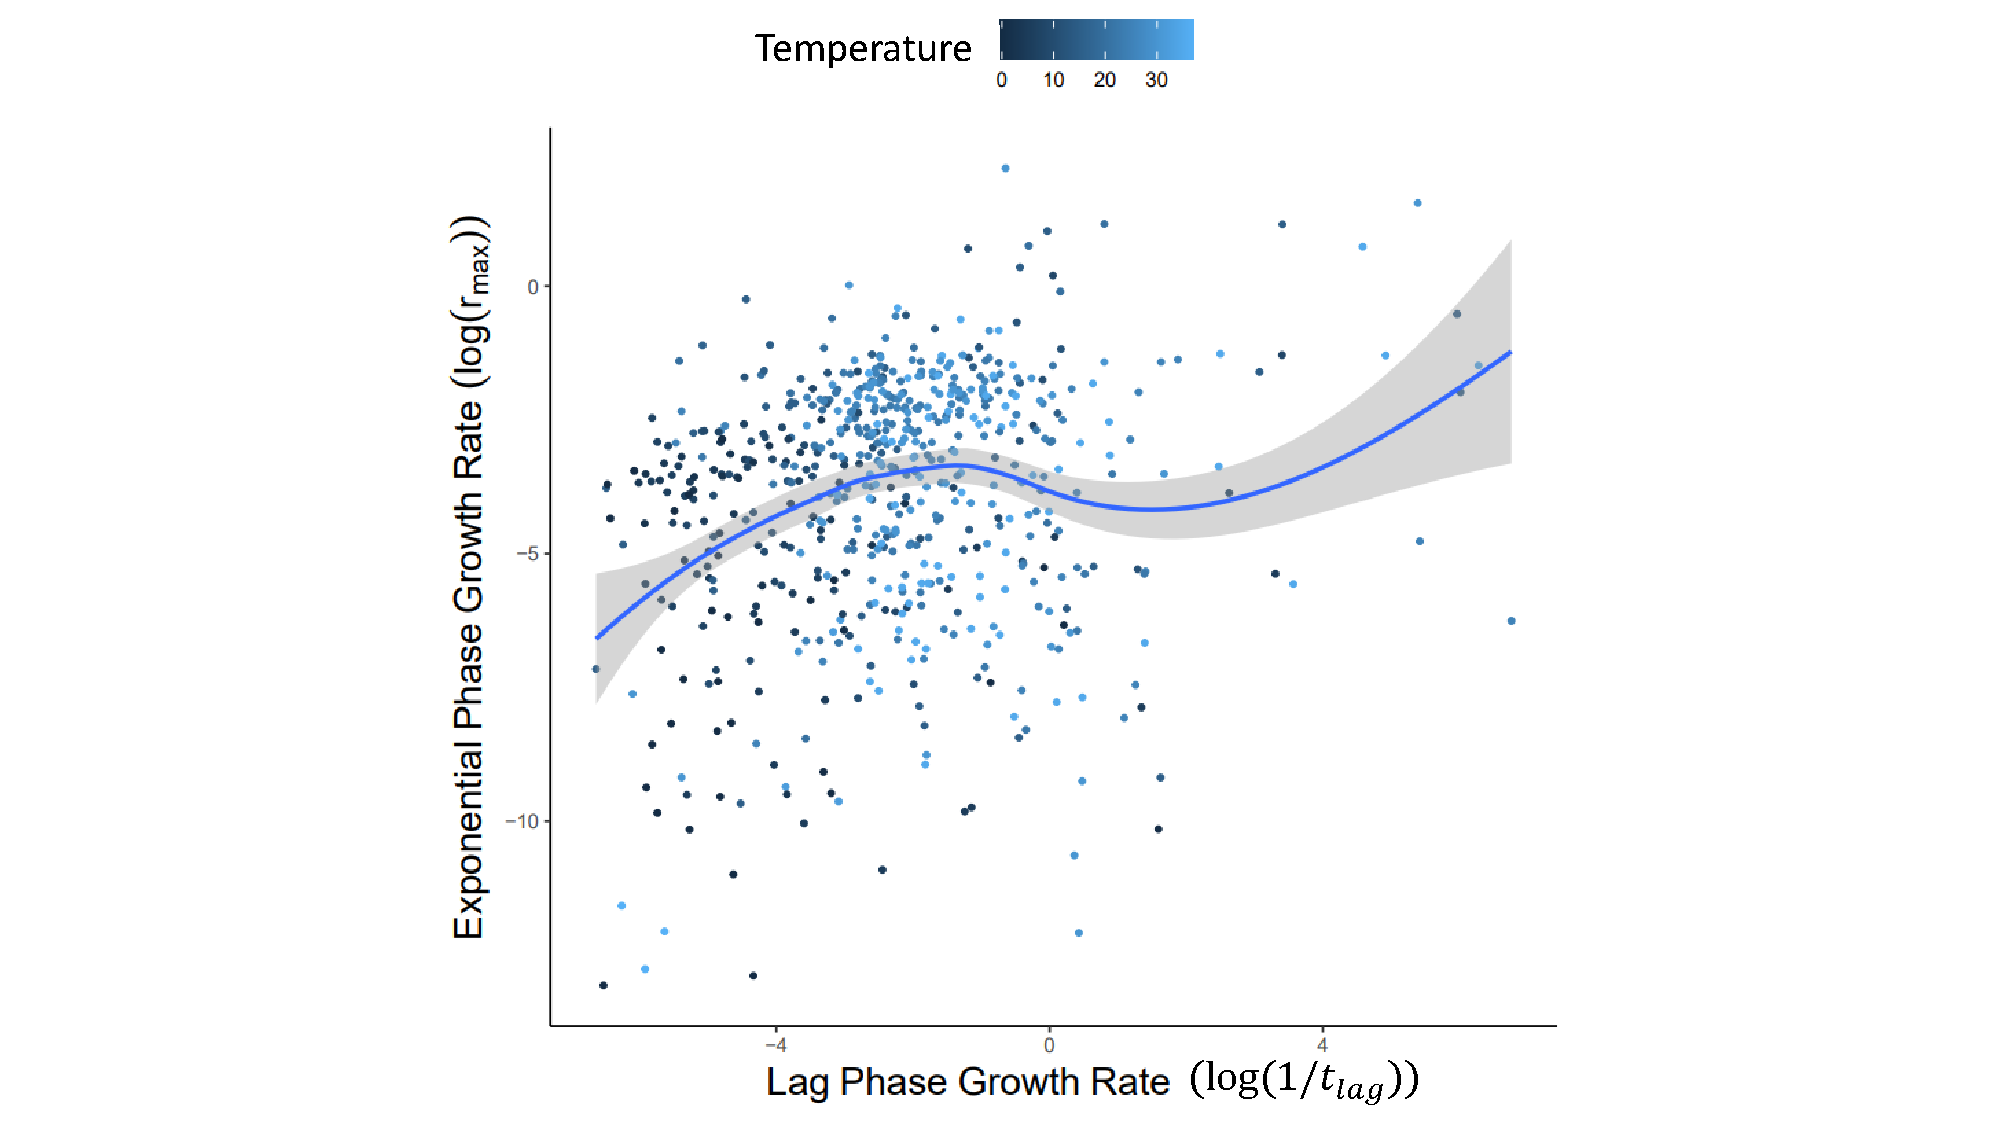
\includegraphics[width=1.1\linewidth]{Plot/log_rt_col_temp.pdf}
%\caption{Scater plot showing the relationship between \(P_{PK}\)(\(r_{max}\)) and %\(P_{lag}\)(\(1/t_{lag}\))}
%\label{fig:log_rt_temp}
%\end{figure}
%figure \ref{fig:log_rt_temp}, the result shows, the metabolic rates between lag and exponential phase do not have trade off, rather, they are positively correlated. \\

% \newpage
% \section{Paper Notes:}


% 1
\subsection{\citep{swinnen2005quantifying}}
the effects of the amplitude of temperature and the pre/post-shift temperature level have on the occurrence and length of a lag phase.\\
conclusion: the (intermediate) lag phase is influenced clearly bythe normal physiological temperature range, contrast to \citep{mellefont2003effect}'s result: independent of amplitude and normal physio-logical range, had little effect on the relative lagphase duration, but negative temperature has effects.\\


% 2
\subsection{On the lag phase and initial decline of microbial growth curves \citep{yates2007lag}}
*intro “daikan”\\
Various models have been proposed for the initial growing phase of bacteria \citep{baranyi1998comparison, baranyi1993non, baranyi1994dynamic, hills1994new, mckellar1997heterogeneous, mckellar2001development}. see review\citep{swinnen2004predictive}(\%3), quantifying lag phase helps prediction\citep{baty2004estimating} 


% 3
\subsection{Predictive modelling of the microbial lag phase: a review \citep{swinnen2004predictive}}
\subsubsection{Intro}
\begin{enumerate}
    \item primary models:
    \begin{enumerate}
        \item deterministic models: baranyi, gompertz
        \item stochastic models: buchanan
    \end{enumerate}
\end{enumerate}

\subsubsection{quantifying lag time}
\begin{enumerate}
    \item define the lag time:
    in my project use this\citep{buchanan1990mathematical} to define t\_lag when the third derivative equals 0. The illustration figure can be found in \citep{zwietering1992comparison}\\
    \item measuring lag time (population/individual)
    \begin{enumerate}
        \item pop: total viable count/ optical density (OD)
        \item individual: \(t\_lag = \tau\) (adaptation time) + DT (doubling time)
        \item OD is rather less accurate in counting the actual cell number in lag phase than plate count. The main problem with OD techniques is that the detection threshold typically corresponds to a bacterial concentration greater than 106 bacteria/ml\citep{begot1996recommendations}(haven't read(HR), cite from\citep{swinnen2005quantifying}). (\%1)
    \end{enumerate}
\end{enumerate}

\subsubsection{factors can influence the duration of the lag phase}
\begin{enumerate}
    \item the <EVN1>:
    temperature, pH..., <EVN1>\&<EVN2>, \(\Delta<EVN1>\) and the rate of the change (\(\Delta<EVN1> / \Delta t\))\\.
    \item the state of the cells
    \item the \textbf{variation} of the populations:
    \begin{enumerate}
        \item if the \textbf{inoculation size} is too small -> the variation between individual cells is higher -> longer lag phase
        \item if the cells are inoculated from the lag/station phase of <EVN1>, -> the variation is higher -> longer lag phase
    \end{enumerate}
\end{enumerate}
    
\subsubsection{existing modelling approaches}
<work(needed to adapt to <ENV2>)> = <rate><lag>
\begin{enumerate}
    \item 
\end{enumerate}


%4
\subsection{\citep{lenski1998evolution}}
(low probability citing)
hitchhick, linkage


%5
\subsection{The lag-phase during diauxic growth is a trade-off between fast adaptation and high growth rate \citep{chu2016lag}}

diauxic/bi-phasic phenomenon, may not suitable of inoculation, cause the diauxic lag may cause if the microorganisms don't allocate more energy into utilize the preferred sugar, which may have advantage of promoting the fitness of organisms, the cost of intraspecific competition will surpass the benefit of earlier preparation of transferring the use of sugar source \\
the explanation of the lag phase: \\
\begin{enumerate}
    \item time required to induce gene[17,18] -> doesn't seem to determining the length of the lag phase
    \item the lag phase is more likely under evolution control[8,19]
    \item unequal distribution of growth rate within population[4,18,21]
\end{enumerate} citation



%6
\subsection{On the duration of the microbial lag phase \citep{vermeersch2019duration}}:
main: what cause the arise of the lag phase, and what factors influence the duration of the lag phase
\subsubsection{the time bacteria needed to adapt to the new environment}
\subsubsection{the past the environment can influence the present}
activation of the respiration as the crucial factor for bacteria to escape the lag phase\\
the unsolved question: why the respiration can be the restrictive factor, there is an assumption that the ATP is the factor (more effective energy source maybe can explain it), there is phenomenon observed by (Perez-Samper et al. 2018) that the drop is more severe in cells that cannot respire. !? how many ways are there for bacteria to repress respiration?
\subsubsection{the variation within the individuals in the population}
it is to say that even in genetically identical population, some individuals adapt faster then some others. \\
original sentence for the first explanation: One simple explanation would be that the lag duration depends on the cell cycle stage a particular cell is in when the carbon source shift happens\\
biological noise: the variation maybe the more favorable strategy if the environment is changing frequently or unpredictable, so that when the environment is changed, there is always some most adaptive individuals can growth immediately. \\


%7
\subsection{Lag Phase Is a Dynamic, Organized, Adaptive, and Evolvable Period That Prepares Bacteria for Cell Division \citep{bertrand2019lag}}
more detail than \%6 \\




hints: you duoshao variation shi keyi bei wuzhong fenlei jieshi de you you duoshao shi bei huanjing jieshi de.\\

will the velocity of adaptation(the duration of the lag phase) influence the carbon gain of the bacteria? \\ 
% (https://onlinelibrary.wiley.com/doi/full/10.1111/btp.12993#btp12993-bib-0053)
\\


% 7
The mechanism of the metabolism happens in the cell when encountering new environment \citep{shimizu2013metabolic}























==================\\ qian bi ji
- Growth Rate and Generation Time of Bacteria, with Special Reference to Continuous Culture
- When is simple enough
- \\



- qian biye lunwen\\



**Natural laws** describe the behaviour of variables: they explain how the variable value(the quality/quantity properties of a variable) would change in corresponding to the other.

pay attention to **the scope of your law and variable** 

natural law deals with variables but pays attention to whether the scope of the laws match the scope of the observations

[in my research: data set (without specific other circumstance criteria) ](https://www.notion.so/9a9c5e460bd14affb77eb4d76eb30160)

you can observe the natural laws by collecting data and spotting a pattern

incomplete laws predict distributions

Chapter 2 - Distributions

Summary: Distributions reveal useful information, but the information is probabilistic.

parametric distribution

natural laws explain how the variable vary which makes distribution an important tool

July 8, 2021 Meeting

model selection: (popProject shoucang jia)\\
== qian wenzhang

can't understand how it infers that the MTE imply 

how could MTE predict the constrain(trade-off) between growth rate and K: as temperature

high growth rates, low life expectancies and low carrying capacity

Method: model fitting

Result:

% \newpage
% \textbf{Work Flow:} \\
\textbf{Code} \\
1. \(install\_package.R\) \\
2. data.R -> \(processed\_data.R\) \\
3. \(model\&fitting\_function.R\) \\
4. \(starting\_value.R -> starting\_value.csv\) \\
5. \(fit\_model.R\) (load data, load \(model\&fitting\_function.R\), load starting\_point.R) \\
6. \(\) \\
7. \(\) \\

%%%%%%%%%%%%%%%%%%%%%%%%%%

%%% *****: 30-40$^{\circ}$C tr positive, thermal response analyses r->HiB holds,t not
% Higher-is-Better hypothesis (HiB hereafter) \citep{angilletta2010thermodynamic}.

%with population size measured in 10 different units: "OD\_595", "N", "mg*C*(g\^-1)", "CFU", "Absorbance (660 nm)", "CFU/g", "microbial Abundance (10\^9 cells)/L", "CGU", "DryWeight" and "Absorbance (600nm) continuous"  
%and Baranyi \citep{baranyi1994dynamic} models using minpack.lm package R language which is based on the Levenberg-Marquardt algorithm.\\
%and Buchanan\citep{buchanan1997simple}(maybe not using stochastic model)


% the E_L is lower means the microbes has lower T_opt evolve to higher optimal trait value, so that when applying the Arrheni  it has lower value. 
% Why use optimal temperature: there is an underlying assumption that we reckon the species is adapted ...